\documentclass[aspectratio=169, 9pt]{beamer}
\usepackage{bbm}
%\usepackage{algorithm2e}
%\usepackage{mathtools}
%\usepackage{graphicx}
%\usepackage{animate}
%\usepackage{hyperref}
\renewcommand\appendixname{Appendix}
%\usepackage{xcolor}
\usepackage[customcolors]{hf-tikz}
%\tikzset{offset def/.style={
%        above left offset={-0.1,0.35},
%        below right offset={0.1,-0.2},
%    },
%    color def/.style={
%        offset def,
%        set fill color=green,
%        set border color=red,
%    },
%}
\usepackage{marvosym}
\usepackage{fontawesome}
\colorlet{rred}{red!80!black}
\colorlet{ggreen}{green!80!black}
\colorlet{grey}{black!50!white}

\usetheme[progressbar=foot]{metropolis}
\metroset{block=fill}
\usepackage{appendixnumberbeamer}
\setbeamercovered{invisible}

\usepackage{booktabs}
%\usepackage[scale=2]{ccicons}
\usepackage[style=authortitle,backend=bibtex]{biblatex}
\addbibresource{biblio.bib}

\usepackage{pgfplots}
\usepgfplotslibrary{dateplot}
\setbeamertemplate{caption}{\raggedright\insertcaption\par}
\setlength{\abovecaptionskip}{-3pt plus 0pt minus 0pt}

%\usepackage{xspace}
\theoremstyle{definition}
\newtheorem{defn}{Definition}
\newtheorem{obs}{Observation}

% math symbols
% Fancy math fonts, requires amsfonts and amsmath
%% Elephant Letters
\newcommand{\A}{\mathbb{A}}
\newcommand{\B}{\mathbb{B}}
\newcommand{\Ch}{\mathbb{C}}
\newcommand{\D}{\mathbb{D}}
\newcommand{\E}{\mathbb{E}}
\newcommand{\F}{\mathbb{F}}
\newcommand{\Gh}{\mathbb{G}}
\newcommand{\Hh}{\mathbb{H}}
\newcommand{\I}{\mathbb{I}}
\newcommand{\J}{\mathbb{J}}
\newcommand{\K}{\mathbb{K}}
\newcommand{\Lh}{\mathbb{L}}
\newcommand{\M}{\mathbb{M}}
\newcommand{\N}{\mathbb{N}}
\newcommand{\Oh}{\mathbb{O}}
\newcommand{\Ph}{\mathbb{P}}
\newcommand{\Q}{\mathbb{Q}}
\newcommand{\R}{\mathbb{R}}
\newcommand{\Sh}{\mathbb{S}}
\newcommand{\T}{\mathbb{T}}
\newcommand{\Uh}{\mathbb{U}}
\newcommand{\V}{\mathbb{V}}
\newcommand{\W}{\mathbb{W}}
\newcommand{\X}{\mathbb{X}}
\newcommand{\Y}{\mathbb{Y}}
\newcommand{\Z}{\mathbb{Z}}

%% Calligrafical Letters
\newcommand{\Ac}{\mathcal{A}}
\newcommand{\BB}{\mathcal{B}}
\newcommand{\CC}{\mathcal{C}}
\newcommand{\DD}{\mathcal{D}}
\newcommand{\EE}{\mathcal{E}}
\newcommand{\FF}{\mathcal{F}}
\newcommand{\GG}{\mathcal{G}}
\newcommand{\HH}{\mathcal{H}}
\newcommand{\II}{\mathcal{I}}
\newcommand{\JJ}{\mathcal{J}}
\newcommand{\KK}{\mathcal{K}}
\newcommand{\LL}{\mathcal{L}}
\newcommand{\MM}{\mathcal{M}}
\newcommand{\NN}{\mathcal{N}}
\newcommand{\OO}{\mathcal{O}}
\newcommand{\PP}{\mathcal{P}}
\newcommand{\QQ}{\mathcal{Q}}
\newcommand{\RR}{\mathcal{R}}
\newcommand{\Sc}{\mathcal{S}}
\newcommand{\TT}{\mathcal{T}}
\newcommand{\UU}{\mathcal{U}}
\newcommand{\VV}{\mathcal{V}}
\newcommand{\WW}{\mathcal{W}}
\newcommand{\XX}{\mathcal{X}}
\newcommand{\YY}{\mathcal{Y}}
\newcommand{\ZZ}{\mathcal{Z}}


\DeclareMathOperator*{\argmin}{argmin}
\DeclareMathOperator*{\argmax}{argmax}


\title{Diffusion Models and an application to DALL-E2\\ 
  \large{Deep Learning and Neural Networks: Advanced Topics}}
\date{March 16, 2023}
\author{Fabio Brau}
\institute{Scuola Superiore Sant'Anna, Pisa.}
% \titlegraphic{\hfill\includegraphics[height=1.5cm]{logo.pdf}}

\setbeamertemplate{background}{%
    \begin{picture}(300,253)
      \hspace{14.45cm}
       
\includegraphics[scale=0.1]{pic/logoretis_noname.png}
   \end{picture}
}
\setbeamercolor{background canvas}{bg=white}
\begin{document}
{\setbeamertemplate{background}{%
    \begin{picture}(300,240)
      \hspace{0.9cm}
       
\includegraphics[scale=0.35]{pic/tecip_logo-ENG.png}
       \hspace{0.5cm}
       
\includegraphics[scale=0.085]{pic/logoretis.png}
   \end{picture}}%
\maketitle
}
\begin{frame}
  \tableofcontents
\end{frame}
\section{Introduction}
\begin{frame}{Generative Models}
  \begin{figure}[h!]
    \centering
    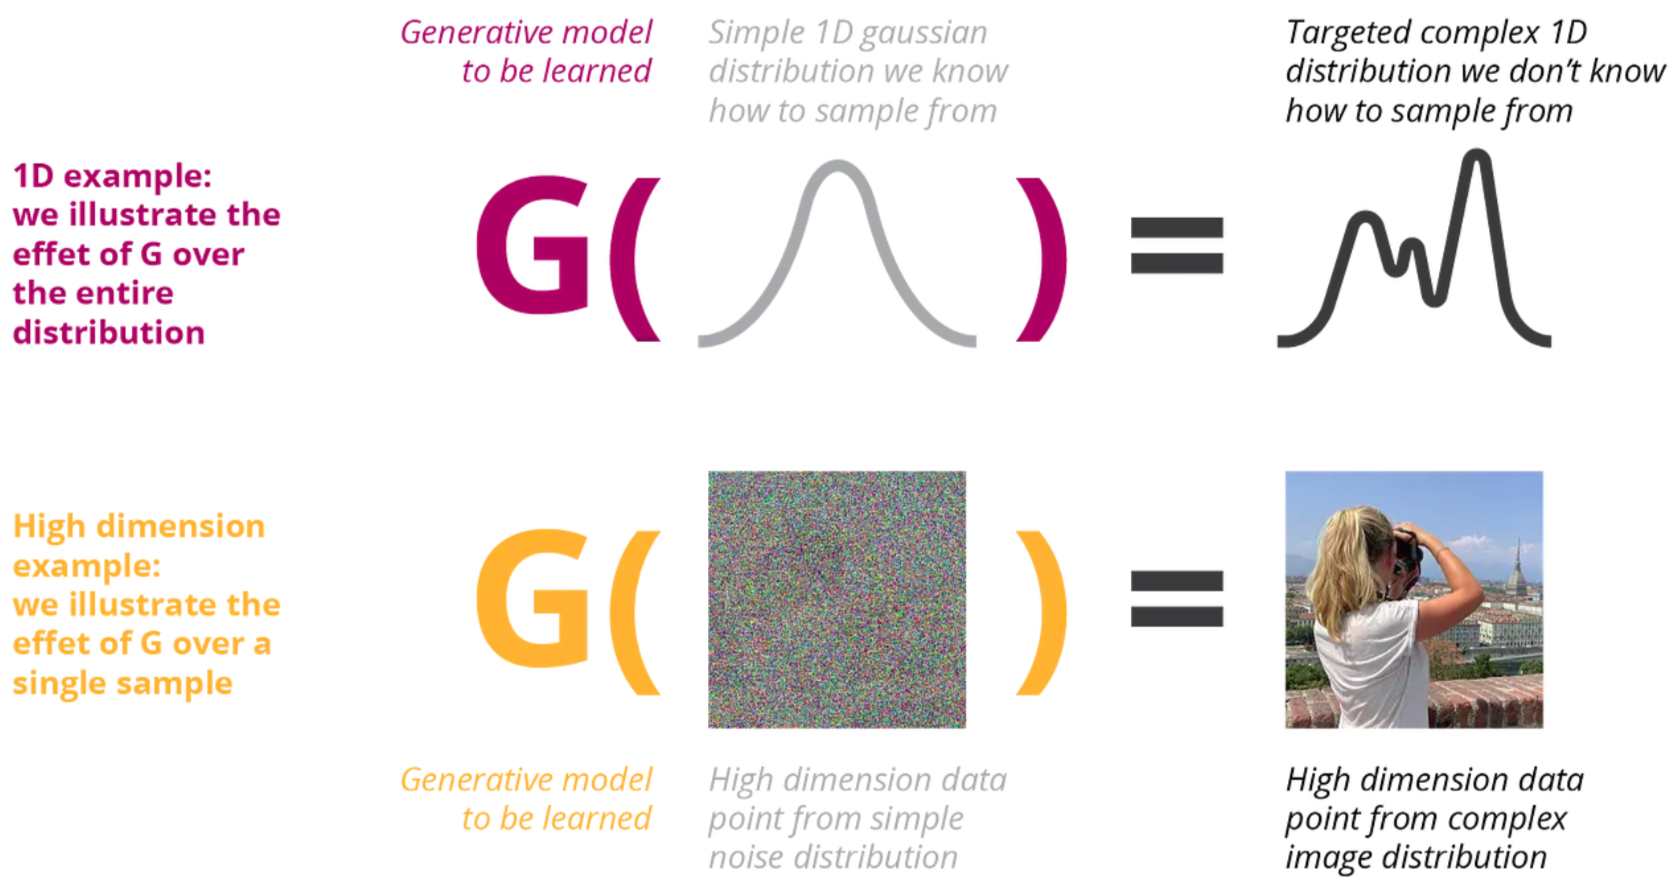
\includegraphics[width=0.75\textwidth]{./pic/generative-models-introa.png}
    \caption{Schema of generative
    models\footnote{\textbf{Credits:} https://towardsdatascience.com/understanding-diffusion-probabilistic-models-dpms-1940329d6048}}
  \end{figure}
\end{frame}
\begin{frame}{Generative Models}
  \begin{figure}[h]
    \centering
    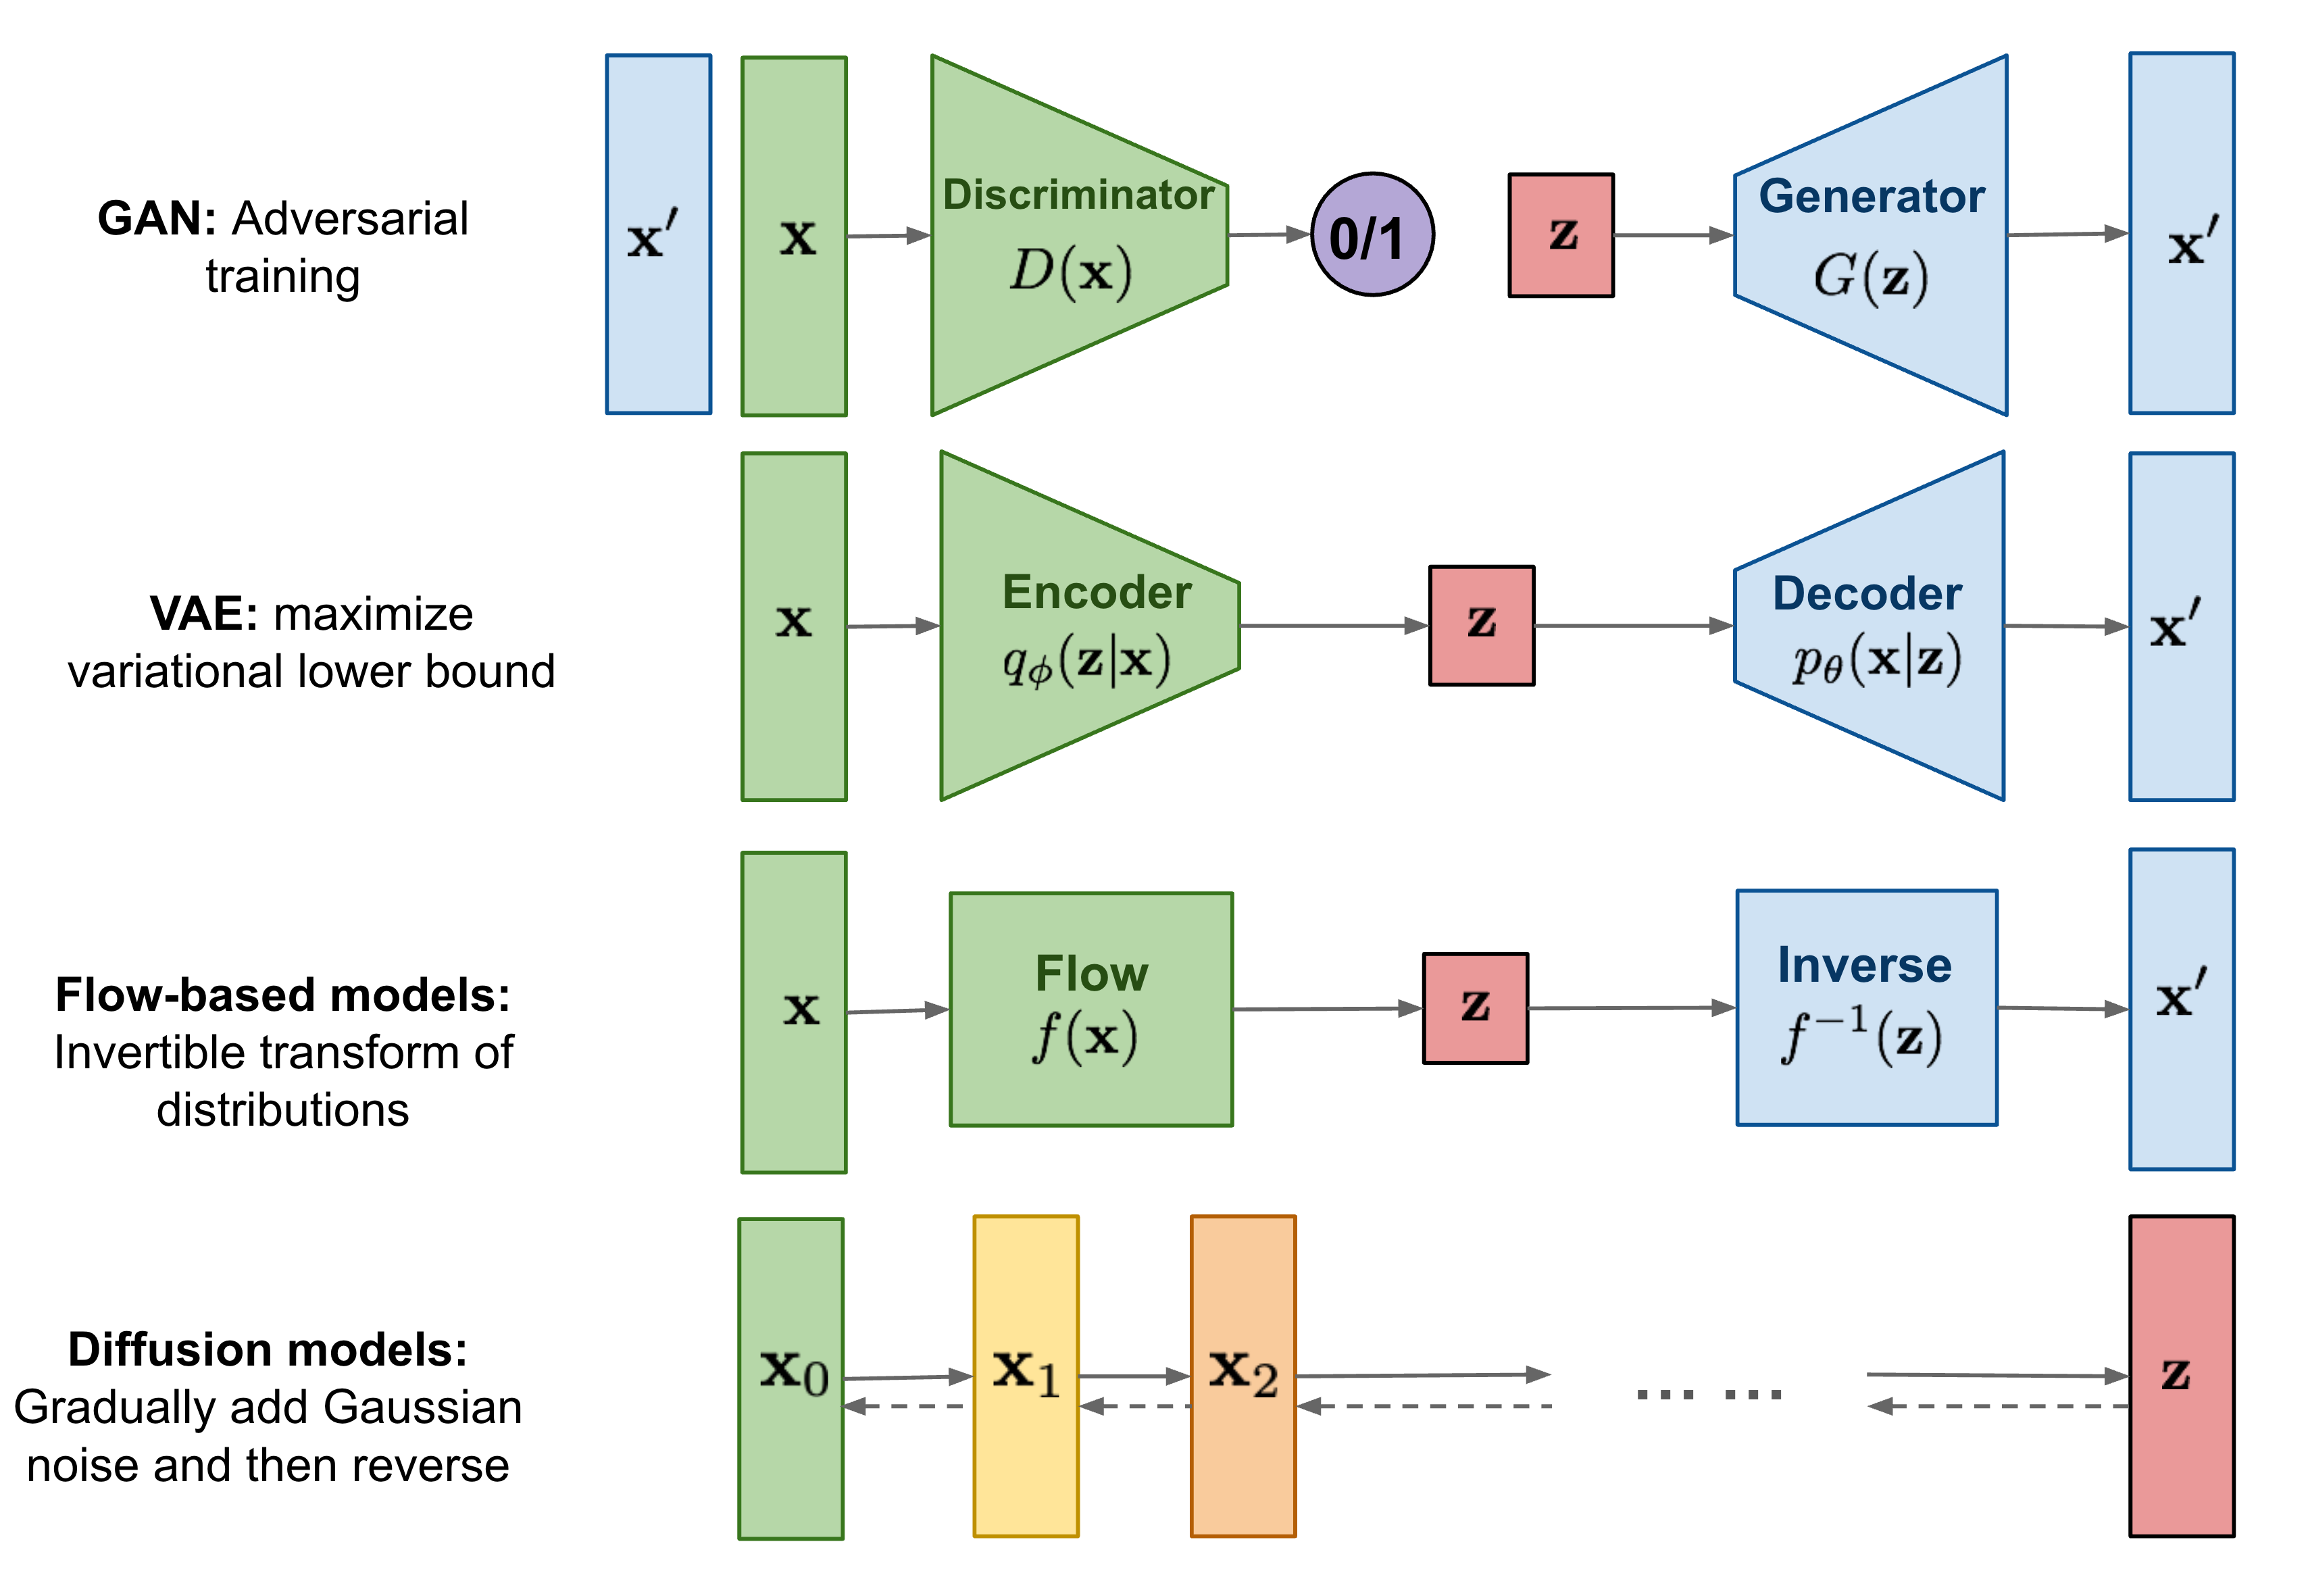
\includegraphics[width=0.65\textwidth]{./pic/generative-overview.png}
    \caption{Overview of different generative
    models\footnote{\textbf{Credits}
  https://lilianweng.github.io/posts/2021-07-11-diffusion-models/}}
  \end{figure}
\end{frame}
\section{Diffusion Models}
\begin{frame}{Overview}
  \begin{center}
    \it
    Diffusion models are generative models that aim at denoising data
  \end{center}
  \begin{figure}[h!]
    \centering
    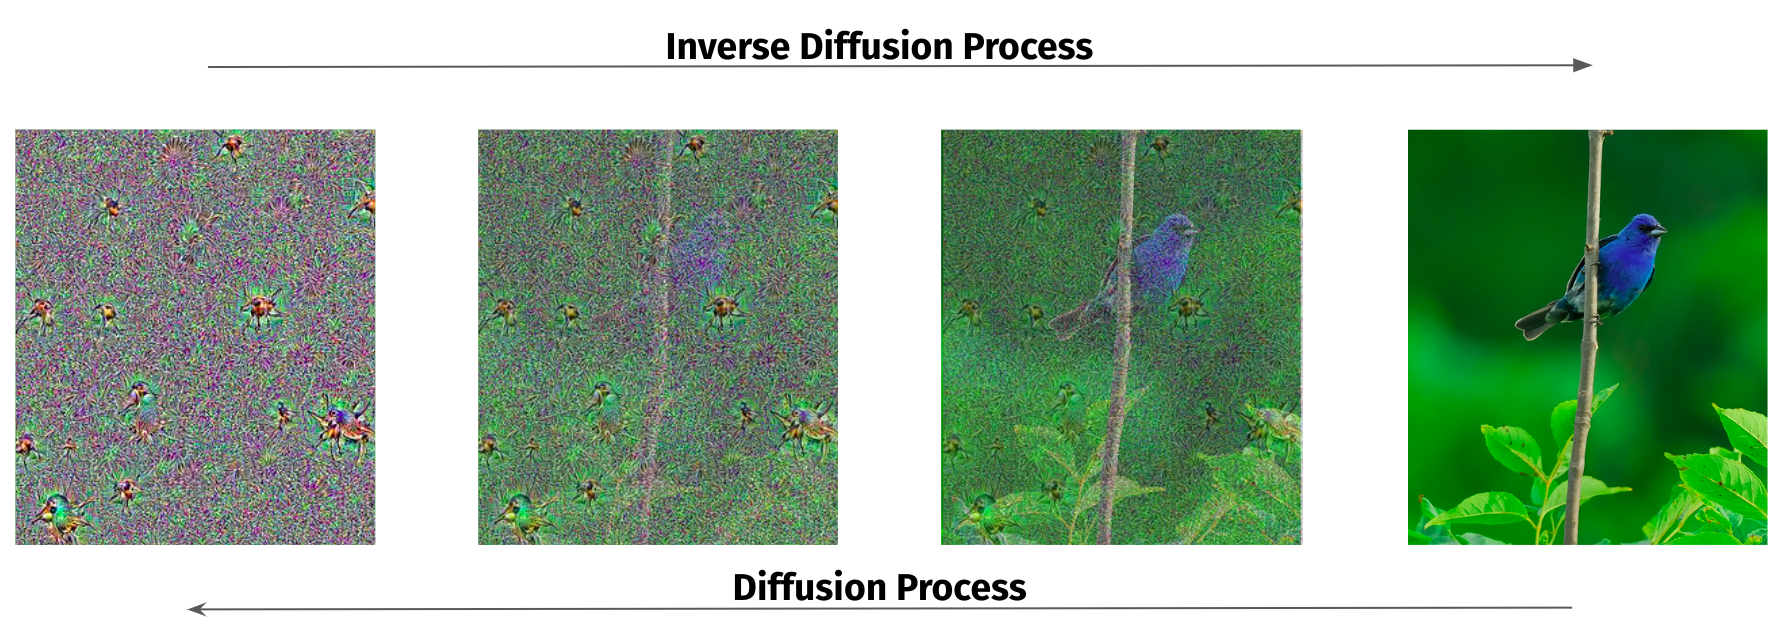
\includegraphics[scale=0.2]{./pic/diffusion_intro.png}
  \end{figure}
\end{frame}
\begin{frame}{Timeline}
\begin{enumerate}
  \item[\bf 2015)] \textit{Deep Unsupervised Learning with Non-equilibrium
  Thermodynamics}. Sohl-Dickstein et al. ICML.\vfill
  \item[\bf 2020)] \textit{Denoising Diffusion Probabilistic Models}.
  Ho et al. NeurIPS.\vfill
  \item[\bf 2021)] \textit{Score-Based Generative Modeling Through SDE}. Song et
    al. ICLR.
\end{enumerate}
\end{frame}

\begin{frame}{Deep Unsupervised Learning using Non-Equilibrium Thermodynamics}
  \begin{figure}[h!]
    \centering
    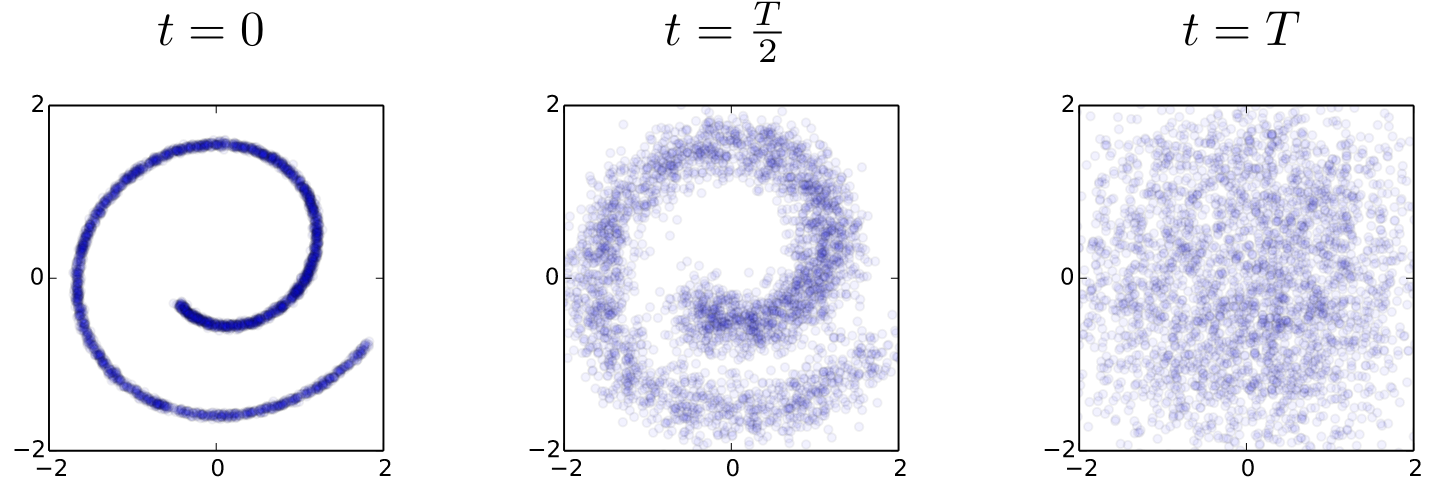
\includegraphics[scale=.23]{./pic/thermodynimc.png}
    \caption{Diffusion process as a \textbf{Markov Chain} with \textbf{Continuous
    State Space} and \textbf{Discrete Time}.\footcite{thermodynamic}}
  \end{figure}
\end{frame}
\begin{frame}{Reminder: Markov Chains with Discrete Time}
\textbf{Informal Definition}\\ 
A sequence of random variables $\xx^{(0)},\xx^{(1)},\cdots,\xx^{(t)},\cdots$,
such that
\begin{itemize}
  \item $\xx^{(t)}\in S$, where $S$ \textbf{State Space}
  \item The future $\xx^{(t+1)}$ depends on the present $\xx^{(t)}$ 
    but not on the past $\xx^{(t-1)}$
\end{itemize}
  \vfill
\begin{columns}
  \begin{column}{0.5\textwidth}
    \begin{center}
      \textbf{Discrete State Space} $S$
    \end{center}
    \begin{figure}[h!]
      \centering
      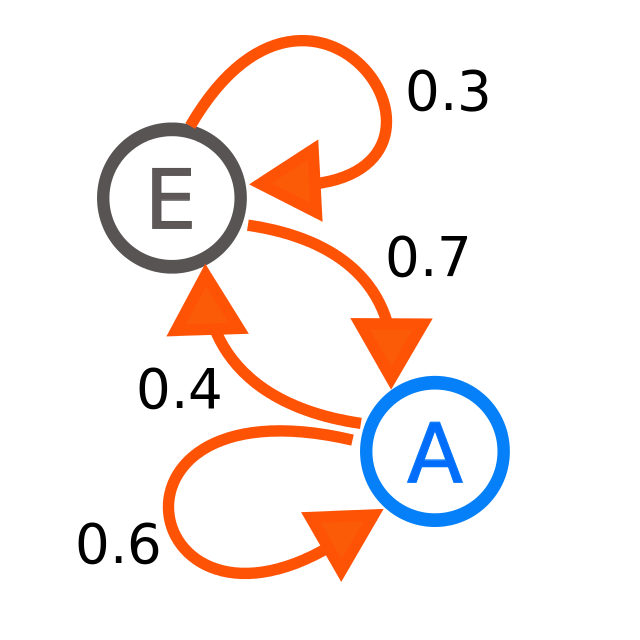
\includegraphics[width=0.5\textwidth, trim=0 0 0
      3cm]{./pic/markov_chain_discrete space.png}\
    \end{figure}
  \end{column}
  \begin{column}{0.5\textwidth}
    \begin{center}
      \textbf{Continuous State Space $S$}
      \begin{figure}[h!]
      \centering
      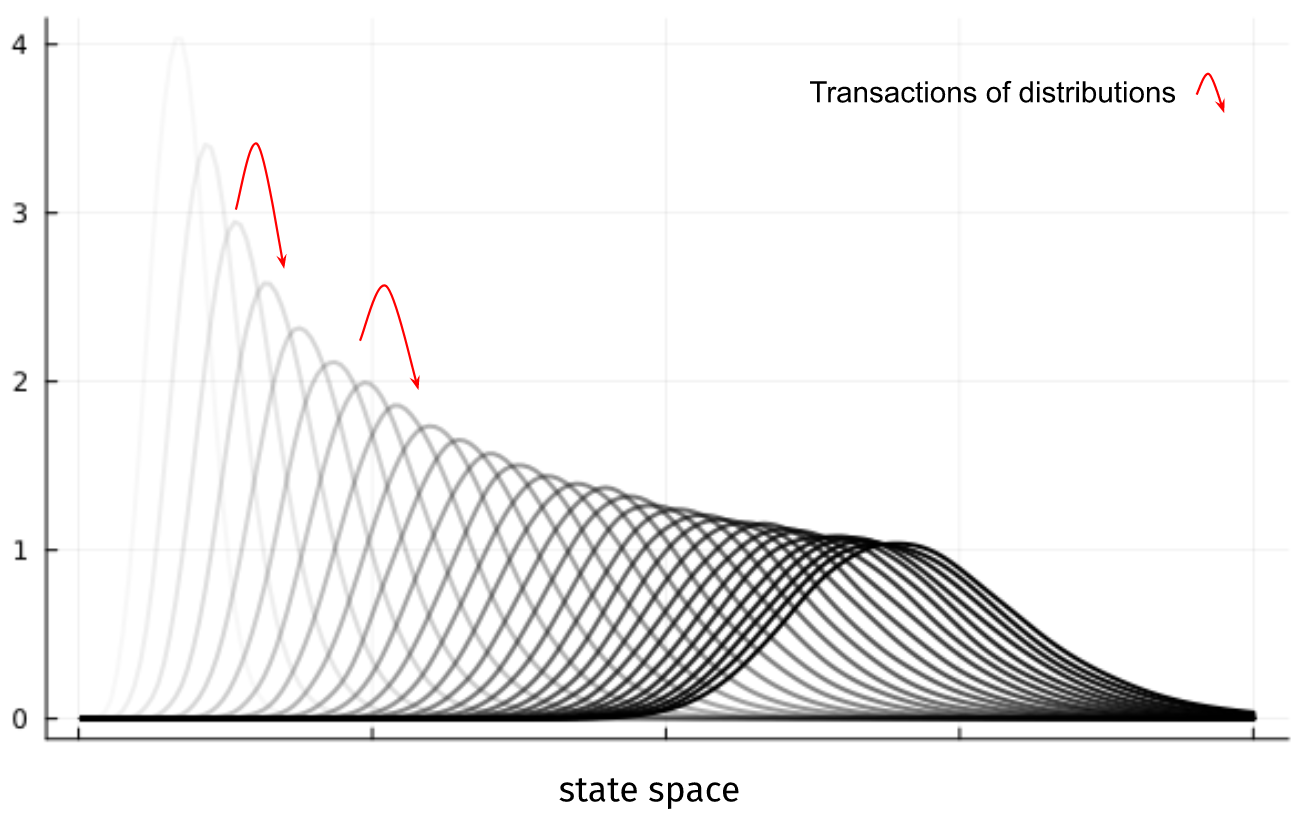
\includegraphics[width=0.75\textwidth, trim=0 0 0 2cm]{./pic/markov_chain_continous space2.png}
    \end{figure}
    \end{center}
  \end{column}
\end{columns}
\end{frame}
\begin{frame}{Reminder: Disrete Time Markov Chain with Discrete State Space}
  \begin{columns}
  \begin{column}{0.6\textwidth}
    \textbf{Definition}\\
    A sequence $\left\{ \xx^{(t)}\right\}_{t\in\N}
    \subseteq S$, a matrix $P=\left( p_{ij} \right)$.
    \vspace{1cm}
    \begin{itemize}
      \item \textbf{Discrete state space}: \(
        S=\left\{ s_0,\cdots,s_n,\cdots \right\}
      \) 
      \vspace{1cm}
    \item \textbf{Markov Property:} $\xx^{(t+1)}$ not dep. $\xx^{(0)},\cdots,\xx^{(t-1)}$.
      \vspace{1cm}

    \item \textbf{Transition Matrix}: \(
        \Ph\left( \xx^{(t+1)}=s_j \vert \xx^{(t)}=s_i\right)=p_{ij}
      \)
    \end{itemize}
  \end{column}
    \begin{column}{0.4\textwidth}
      \onslide<2>{%
      \begin{block}{\textbf{$P$ is a stochastic matrix!}}
        \[
          \forall i,\quad \sum_{j\in\N}p_{ij}=1
        \]
      \end{block}
      \vspace{1cm}
      \begin{figure}[h!]
        \centering
        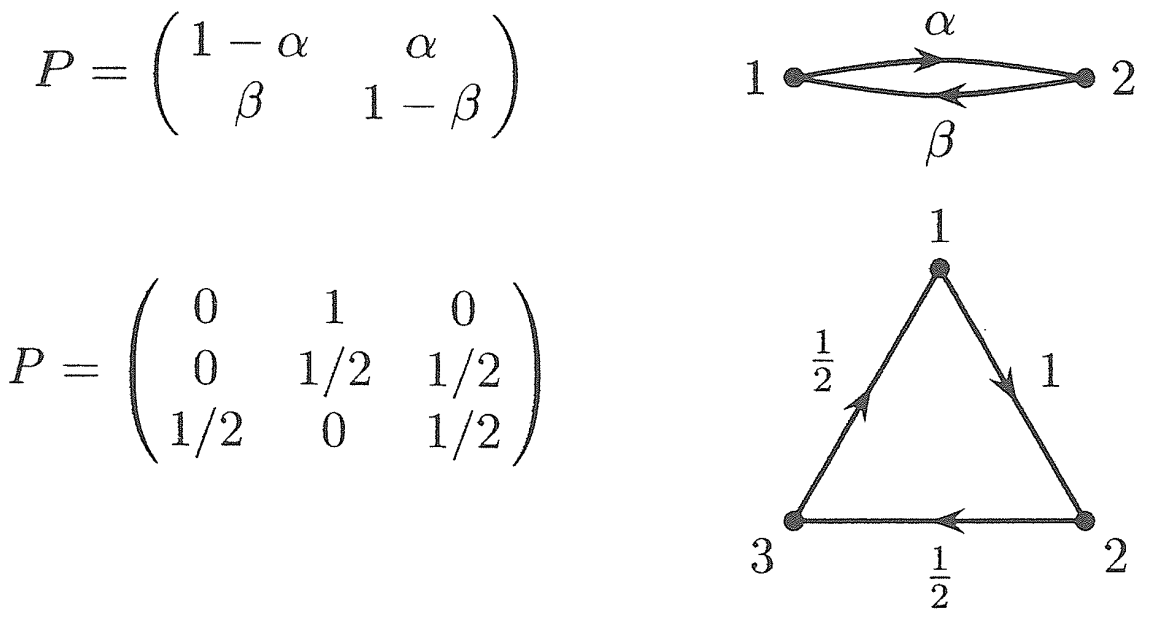
\includegraphics[width=0.75\textwidth]{./pic/mcdt_discrete_space.png}
      \end{figure}
    }
  \end{column}%
  \end{columns}
\end{frame}
\begin{frame}{Reminder: DTMC with Continuous State Space}
  Let assume $\xx,\yy\in S$ where $S$ continuous state space (e.g.
  $S=\R^d$).\\
  \vfill
  \begin{block}{\textbf{Joint Distribution} $p(\xx,\yy)$}
  \[
    \Ph\left( \xx\in A\,\vert\,\yy\in B \right)=
    \int_A\int_B p\left( \xx,\yy \right)\,d\xx\,d\yy
  \]
\end{block}
\begin{block}{\textbf{Transactional Kernel} $p(\xx\,\vert\,\yy)$}
    \[
      p\left( \xx,\yy \right) = p(\xx\,\vert\,\yy)\,p\left( \yy \right)
    \]
  \end{block}
  \begin{block}{\textbf{Marginal Distribution} $p(\xx)$}
    \[
      p\left( \xx \right)=\int_S p\left( \xx,\yy \right)\,d\yy = \int_S
      p(\xx\,\vert\,\yy)\,p\left( \yy\right)\,d\yy 
    \]
  \end{block}
\end{frame}
\begin{frame}{Forward Diffusion Process}
  \begin{center}
    ``Adding noise to data\ldots''
  \end{center}
  \begin{itemize}
    \item \textbf{Data Distribution}: $\xx^{(0)}\sim q$
      \hfill\onslide<2->{{\color{red} Not Analytic!!}}
    \item \textbf{Transaction Kernel}: $q\left( \xx^{(t)}\,\vert\,\xx^{(t-1)}
      \right)=\NN\left( \xx^{(t)};\sqrt{1-\beta_t}\xx^{(t-1)}; \beta_t I \right)$
    \item \textbf{Variance Scheduler}: $0<\beta_1<\cdots<\beta_T< 1$ 
  \end{itemize}
  \begin{figure}[h!]
    \centering
    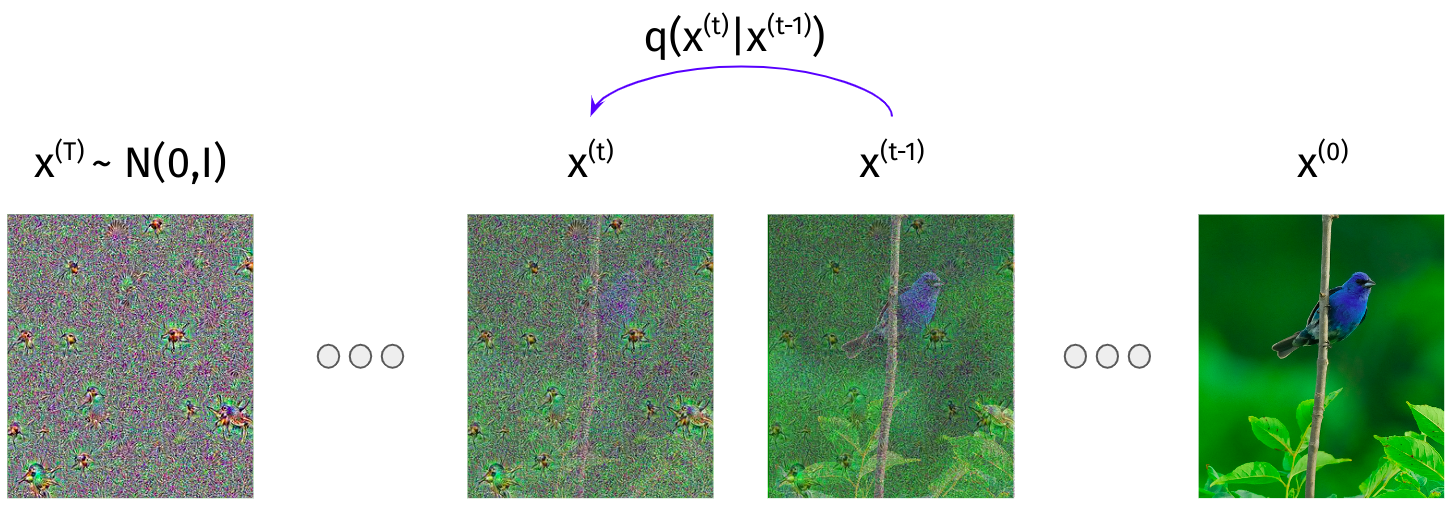
\includegraphics[width=0.75\textwidth]{./pic/forward-diffusion.png}
  \end{figure}
\end{frame}
\begin{frame}{Forward Diffusion Process: Explicit Representation}
  \[
    \xx^{(t)}=\sqrt{1-\beta_t}\,\xx^{(t-1)} +
    \sqrt{\beta_t}\,\varepsilonb_t,\quad
    \varepsilonb_t\sim\NN(0,I)
  \]
  \begin{block}{Observation: Many small noisy steps $\approx$ Large Noisy
    step}
    \[
      \xx^{(t)} = \sqrt{1-\alpha_t}\, \xx^{(0)} + \sqrt{\alpha_t}
      \varepsilonb,\quad \varepsilonb\sim\NN(0,I)
    \]
    where
    \[
      \alpha_t = 1-\prod_{i=0}^t(1-\beta_i)
    \]
  \end{block}
\end{frame}
\begin{frame}{Forward Diffusion Process: Distribution Representation}
  \begin{center}
    Markov property allows breaking up distributional Representation\ldots
  \end{center}
  \begin{equation}
    \begin{aligned}
    q(\xx^{(0)},\ldots,\xx^{(T)}) &= q\left( \xx^{(T)}\,|\,
      \xx^{(0)},\ldots,\xx^{(T-1)} \right)\,q\left(
      \xx^{(0)},\ldots,\xx^{(T-1)} \right)\\
      \pause
      &= q\left(\xx^{(T)}\,\vert\, \xx^{(T-1)}\right) q\left(
      \xx^{(0)},\ldots,\xx^{(T-1)} \right)\\
      &\vdots\\
    \end{aligned}
  \end{equation}
  \pause
  \begin{block}{Distributional Representation}
    \[
      q(\xx^{(0)},\ldots,\xx^{(T)})= q(\xx^{(0)})\prod_{t=1}^T q\left(
          \xx^{(t)}\,\vert\,\xx^{(t-1)}
        \right)
    \]
  \end{block}
\end{frame}
\begin{frame}{Reverse Diffusion Process}
  \onslide<2->{%
  \textbf{\color{blue}Fixed Forward Process}
  {\color{blue}\footnotesize
  \[
    \begin{aligned}
      & \mbox{Initial Distribution} &\hspace{5cm} &\mbox{Gaussian Transaction
      Kernel}\\
     &q(\xx^{(0)})& & 
     q\left( \xx^{(t)}\,\vert\,\xx^{(t-1)}\right)=
     \NN\left(\xx^{(t)};\sqrt{1-\beta_t}\xx^{(t-1)}; \beta_t I \right)
    \end{aligned}
  \]}}
  \begin{figure}[h!]
    \centering
    %\includegraphics<1>[clip, width=\textwidth, trim=0 6.3cm 0 4.5cm]{./pic/reverse-diffusion.png}%
    %\includegraphics<2>[width=\textwidth,trim=0 6.3cm 0 4.5cm]{./pic/reverse-diffusion.png}
    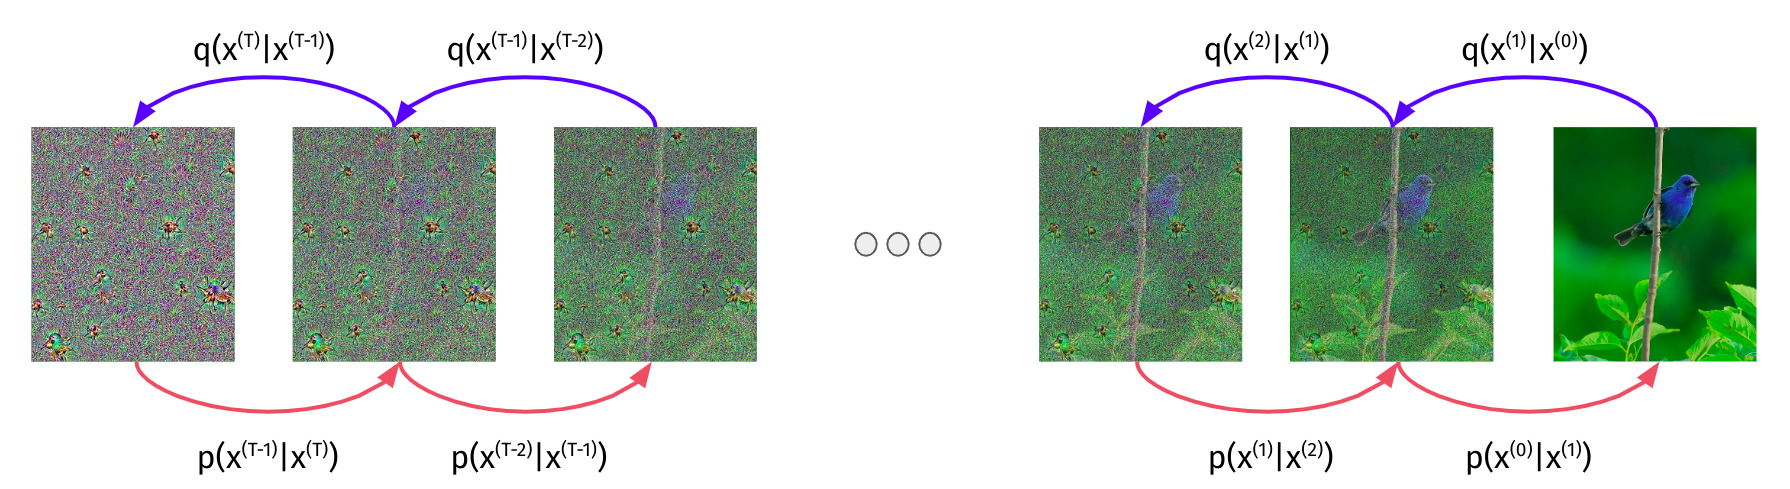
\includegraphics[width=\textwidth, trim=0 1cm 0 2cm]{{./pic/reverse-diffusion-2.png}}%
  \end{figure}
  \vfill
  \onslide<3->{%
  {\color{rred}\footnotesize
  \[
    \begin{aligned}
      & \mbox{Initial Distribution}& \hspace{1cm}\mbox{Approximation of}
      &\hspace{1cm}&\mbox{Gaussian Kernel with parameters}&\\
      &p(\xx^{(T)})\sim\NN(0,I)& q(\xx^{(t-1)}\,\vert\,\xx^{(t)})&&
      p_\theta(\xx^{(t-1)}\,\vert\, \xx^{(t)})=
      \NN\left(\xx^{(t-1)};\mub_\theta\left(\xx^{(t)},t
      \right),\Sigmab_\theta\left(\xx^{(t)},t \right)\right)&
    \end{aligned}
  \]} \textbf{\color{rred}Learned Reverse Process}}
\end{frame}
\begin{frame}{Reverse Diffusion Process}
  \begin{minipage}[t]{0.45\textwidth}
    \begin{center}
      \bf 
      Forward Diffusion Process
    \end{center}
    \begin{equation*}
      \begin{aligned}
        q(\xx^{(0)}) &\quad\mbox{Data Distribution}\\
        q(\xx^{(0\ldots T)})&= q(\xx^{(0)})\prod_{t=1}^T q\left(
          \xx^{(t)}\,\vert\,\xx^{(t-1)}\right)\\
      \end{aligned}
    \end{equation*}
  \end{minipage}\hfill%
  \begin{minipage}[t]{0.45\textwidth}
    \begin{center}
      \bf 
      Reverse Diffusion Process
    \end{center}
    \begin{equation*}
      \begin{aligned}
        q(x^{(T)}) &= \NN(0,I)\\
          q(\xx^{(0\ldots T)})&= q(\xx^{(T)})\prod_{t=1}^T q\left(
          \xx^{(t-1)}\,\vert\,\xx^{(t)}\right)
      \end{aligned}
    \end{equation*}
  \end{minipage}
  \pause
  \begin{block}{Theorem. Reverse of Gaussian DP is $\approx$ Gaussian DP\footcite{thermodynamic}}
    If $|\beta_i-\beta_{i+1}|\approx 0$, i.e.\ diffusion \textbf{slow
    enough}, then% $q\left( \xx^{(t)}\,\vert\,\xx^{(t-1)} \right)=\NN\left( \xx^{(t)};\sqrt{1-\beta_t}\xx^{(t-1)}; \beta_t I \right)$ is such that
    \[
      q(\xx^{(t-1)}\,\vert\, \xx^{(t)}) 
      \approx \NN\left(\xx^{(t-1)};\,\onslide<3->{\tikzmarkin{z1}} 
        \mub_\theta\onslide<3->{\tikzmarkend{z1}}\left(
        \xx^{(t)},t \right),\,
        \onslide<3->{\tikzmarkin{z2}}\Sigmab_\theta\onslide<3->{\tikzmarkend{z2}}\left(
    \xx^{(t)},t \right)\right)
    \]
  \end{block}
  \onslide<3->{\tikzmarkin[below right offset={0.,-0.2}, above left
    offset={0.,0.4}]{b} Mean $\mub_\theta$ and covariance
  $\Sigmab_\theta$ have to be learned!!\tikzmarkend{b}}
\end{frame}
\begin{frame}{Visualization of Diffusion Process: 2D dimensional case}
  \begin{figure}[h]
    \centering
    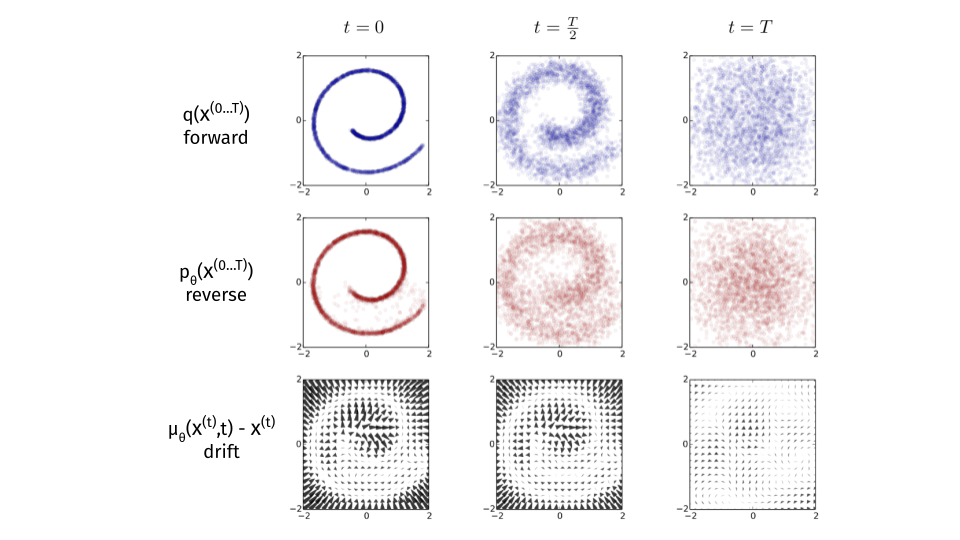
\includegraphics[width=0.75\textwidth]{./pic/summary-forw-reverse.png}\footcite{thermodynamic}
  \end{figure}
\end{frame}
\begin{frame}{Training of $\mub_\theta$ and  $\Sigmab_\theta$}
  \begin{columns}
  \begin{column}{0.45\textwidth}
    \begin{center}
      \bf Goal
    \end{center}
    Search for the best parameters $\theta$ 
    \[
      q(\xx^{(0)}) \approx p_\theta(\xx^{(0)})
    \]
      where $\xx^{(0)}\,\cdots,\,\xx^{(T)}$ diffusion process
      \vspace{1cm}
      \begin{block}{Estimated Reverse Process}
    \[
      \begin{aligned}
        & p_\theta(\xx^{(T)}) = \NN\left( \xx^{(T)}; 0, I \right)\\
        & p_\theta(\cdot\,\vert\, \xx^{(t)})=
        \NN\left(\mub_\theta\left(\xx^{(t)},t \right),
          \Sigmab_\theta\left(\xx^{(t)},t \right)\right)
      \end{aligned}
    \]
  \end{block}
  \end{column}
  \begin{column}{0.45\textwidth}
    \onslide<2->{%
      \begin{center}
        \bf Method
      \end{center}
      Minimize the \textit{Kullback–Leibler} Divergence
      \[
        \onslide<3->{\tikzmarkin{a13}(0.1,-0.4)(-0.1,0.55)}%
        D_{KL}(q\,||\,p_\theta):=\int q(\xx^{(0)})\log\left(
        \frac{q(\xx^{(0)})}{p_\theta(\xx^{(0)})}\right)\,d \xx^{(0)}
        \onslide<3->{\tikzmarkend{a13}}
      \]}
      \onslide<3->{%
        \begin{center}
          \textbf{Easy??}\\
      \end{center}
      }
      \begin{columns}
        \begin{column}{0.45\textwidth}
          \onslide<4->{%
            \begin{center}
              \tikzmarkin{nope}\textbf{No.} $q(\xx^{(0)})$ is analytically
              intractable!!\hspace{1em}\tikzmarkend{nope}
            \end{center}
        }
        \end{column}\hspace{0.5cm}%
        \begin{column}{0.35\textwidth}
          \visible<4->{%
          \begin{figure}[h]
            \centering
            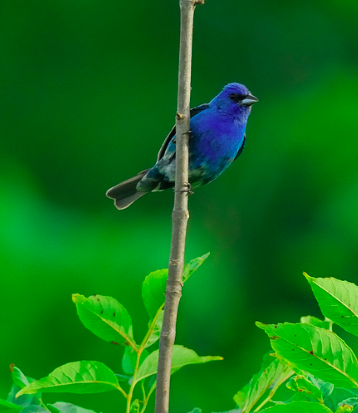
\includegraphics[width=\textwidth]{./pic/sample.png}%
          \end{figure}
        }%
        \end{column}
      \end{columns}
    \end{column}
  \end{columns}
\end{frame}
\begin{frame}{Training of $\mub_\theta$ and  $\Sigmab_\theta$}
  \begin{center}
    \textbf{Goal: Deduce a tractable loss function}
  \end{center}
    \[
      \tikzmarkin{a1}(0.1,0.6)(-0.1,-0.5)D_{KL}(q\,||\,p_\theta):=\int q(\xx^{(0)})\log\left(
      \frac{q(\xx^{(0)})}{p_\theta(\xx^{(0)})}\right)\,d
      \xx^{(0)}\tikzmarkend{a1}
    \]
    \vfill
    \pause
    \begin{center}
      \bf
      Simplification I: Minimize the Cross Entropy
    \end{center}
    %\[
    %D_{KL}\left( q(\xx^{(0)})||p_\theta(\xx^{)0)} \right) =
    %\visible<2>{\int q(\xx^{(0)})\log(q(\xx^{(0)})\,d\xx^{(0)}+
    %  \int-q(\xx^{(0)})\log(p_\theta(\xx^{(0)}))\,d\xx^{(0)}}
    %\visible<3->{\underbrace{\int q(\xx^{(0)})\log(q(\xx^{(0)})\,d\xx^{(0)}}_{-\Hh\left(
    %  q(\xx^{(0)}\right)} + 
    %\underbrace{\int-q(\xx^{(0)})\log(p_\theta(\xx^{(0)}))\,d\xx^{(0)}}_{L_{CE}(p_\theta)}}
    %\]
    \[
    D_{KL}\left( q(\xx^{(0)})||p_\theta(\xx^{)0)} \right) =
    \onslide<3->\underbrace{\onslide<2->%
    \int q(\xx^{(0)})\log(q(\xx^{(0)})\,d\xx^{(0)}\onslide<3->}_{-\Hh\left(
        q(\xx^{(0)}\right)} \onslide<2->+ 
    \onslide<3->\underbrace{\onslide<2->%
  \int-q(\xx^{(0)})\log(p_\theta(\xx^{(0)}))\,d\xx^{(0)}\onslide<3->}_{L_{CE}(p_\theta)}
    \]
\end{frame}
\begin{frame}{Training of $\mub_\theta$ and  $\Sigmab_\theta$}
  \begin{center}
    \bf
    Minimize the Cross Entropy Loss
  \end{center}
    \[
      \tikzmarkin{a2}(0.1,0.6)(-0.1,-0.5)L_{CE}(\,p_\theta(\xx^{(0)}):=-\int
        q(\xx^{(0)})\log\left( p_\theta(\xx^{(0)})\right)\,d
      \xx^{(0)}\tikzmarkend{a2}
    \]
    \pause
    \begin{block}{Observation: Marginal Distribution}
      \[
        %\tiny
        p_\theta(\xx^{(0)})=\int p_\theta(\xx^{(0\ldots T)})\,
        d\xx^{(1\ldots T)}
      \]
    \end{block}
    \pause
    \begin{center}
      \bf
      Simplification II: Jensen Inequality
    \end{center}
    \[
      L_{CE}(p_\theta) \le - \E_{q(\xx^{(0\ldots T)})}\left[ \log
      \frac{q(\xx^{(1\ldots T)}\,\vert\, 
    \xx^{(0)})}{p_\theta(\xx^{(0\ldots T)})}\right]
    \]
\end{frame}
\begin{frame}{Training of $\mub_\theta$ and  $\Sigmab_\theta$}
  \begin{minipage}[t]{0.75\textwidth}
\ldots after some algebraic steps :)
  \begin{center}
    \bf
    Reformulated Loss Function
  \end{center}
  \[
    \LL = \LL_T + \sum_{t=1}^{T-1}\LL_t + \LL_0
  \]
  where, 
  \[
    \begin{aligned}
      \LL_T &= \E_{q(\xx^{(0\ldots T)})}\left[ D_{KL}\left(
      q(\xx^{(T)}\,\vert\, \xx^{(0)}) \quad||\quad p_\theta(\xx^{(T)}) \right)
    \right] \\
     \LL_t &= \E_{q(\xx^{(0\ldots T)})}\left[ D_{KL}\left(
        q(\xx^{(t)}\,\vert\, \xx^{(t+1)},\xx^{(0)}) \quad||\quad
      p_\theta(\xx^{(t)}\,\vert\, \xx^{(t+1)}) \right)
    \right]
    \\
    \LL_0 &= \E_{q(\xx^{(0\ldots T)})}\left[ p_\theta(\xx^{(0)}\,\vert\, \xx^{(1)}) \right]
  \end{aligned}
  \]
\end{minipage}\hfill%
\begin{minipage}[t]{0.20\textwidth}
  \vspace{4cm}
  \textbf{Note.}\\
  $\LL_T$ is constant.\\
  $\LL_0,\,\LL_t$ explicit.\\
\end{minipage}\\
 % \tikzmarkin{a3}All the expectations can be \textbf{explicitly} calculated
 % and only depends on $\theta$!!\tikzmarkend{a3}
\end{frame}
\begin{frame}{Neural Network that estimate $\mub_\theta$ and
  $\Sigmab_\theta$}
  \begin{figure}[h!]
    \centering
    \includegraphics<1>[width=0.45\textwidth]{./pic/diff_net_1.png}%
    \includegraphics<2>[width=0.45\textwidth]{./pic/diff_net_2.png}%
  \caption{Proposed Neural Network for CIFAR10 image generation. T=1000}
  \end{figure}
\end{frame}
\begin{frame}{Sampling or Generative Stage}
  \begin{figure}[h]
    \centering
    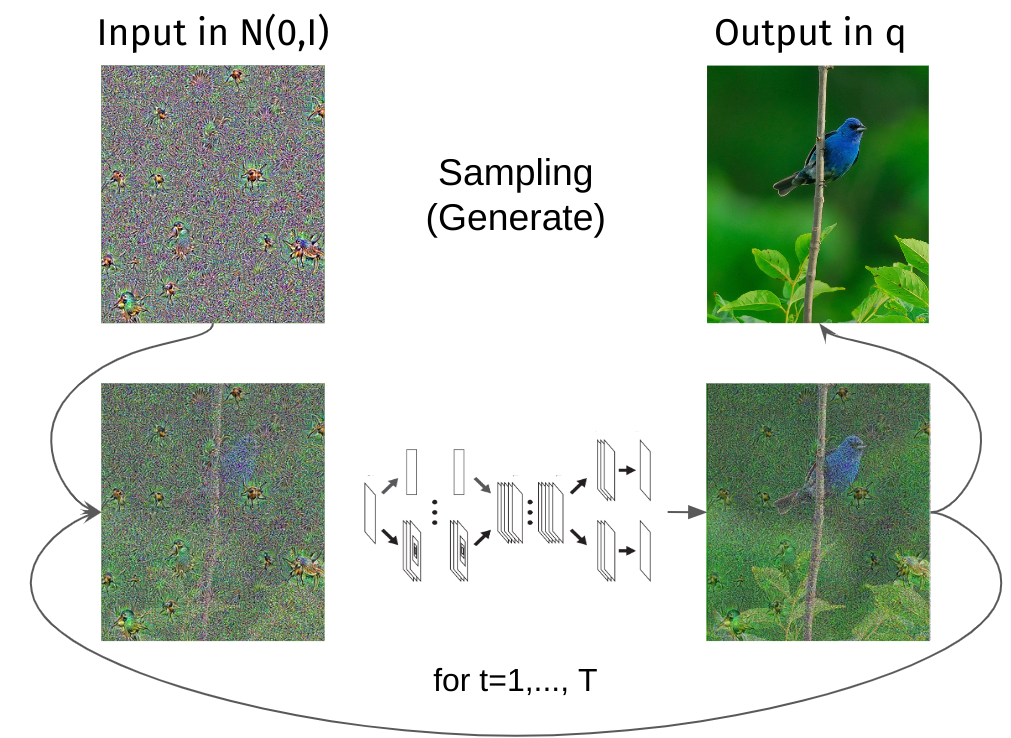
\includegraphics[width=0.5\textwidth]{./pic/sampling.png}
  \end{figure}
\end{frame}
\begin{frame}{Experiments\footcite{thermodynamic}}
  \begin{minipage}[h!]{0.5\textwidth}
    \begin{center}
      \bf
      Bark Dataset
    \end{center}
    \begin{figure}[h!]
      \centering
      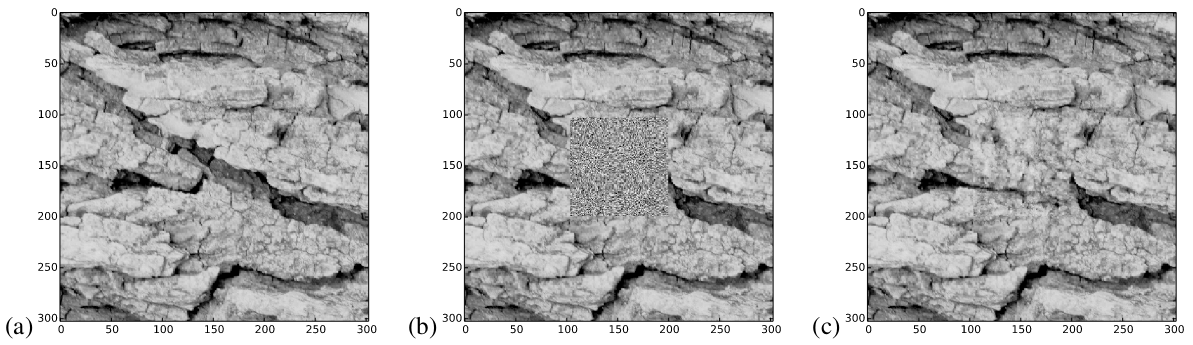
\includegraphics[width=\textwidth]{./pic/bark.png}
    \end{figure}
  \end{minipage}\hfill%
  \begin{minipage}[h!]{0.5\textwidth}

    \begin{center}
      \bf MNIST
    \end{center}
    \begin{figure}[h!]
      \centering
      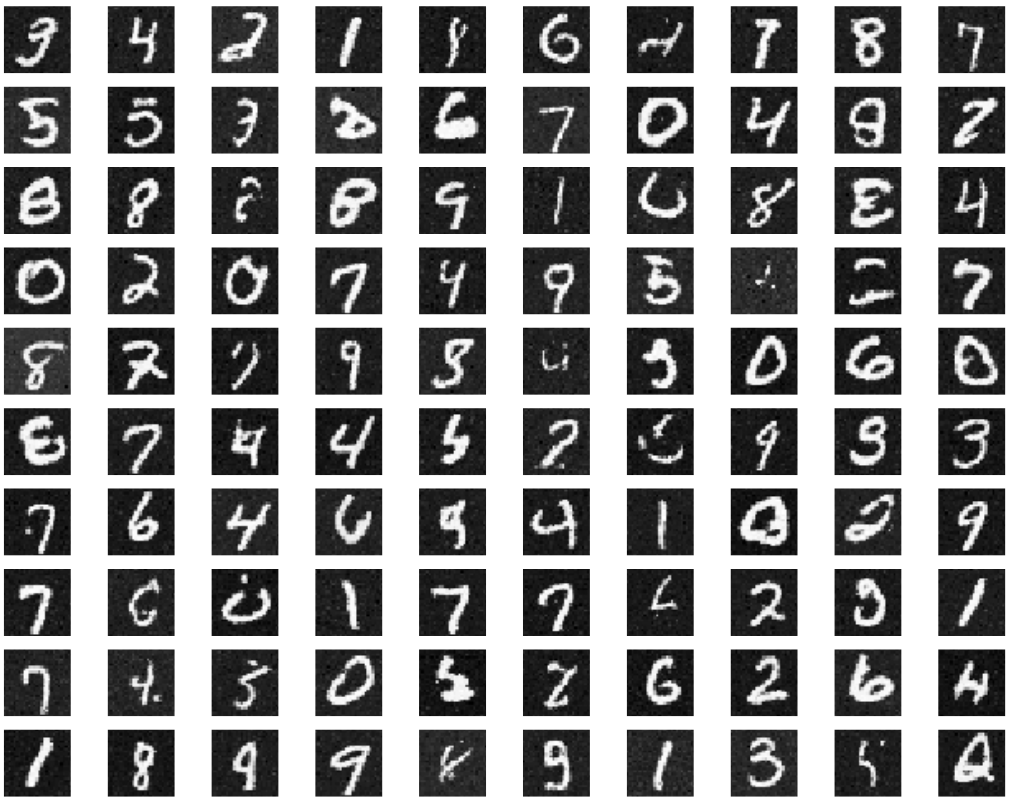
\includegraphics[width=0.75\textwidth]{./pic/mnist_thermo.png}
    \end{figure}
  \end{minipage}
\end{frame}
\begin{frame}{Experiments\footcite{thermodynamic}}
  \begin{minipage}[h!]{0.5\textwidth}
    \begin{center}
      \bf CIFAR10 (original)
    \end{center}
    \begin{figure}[h!]
      \centering
      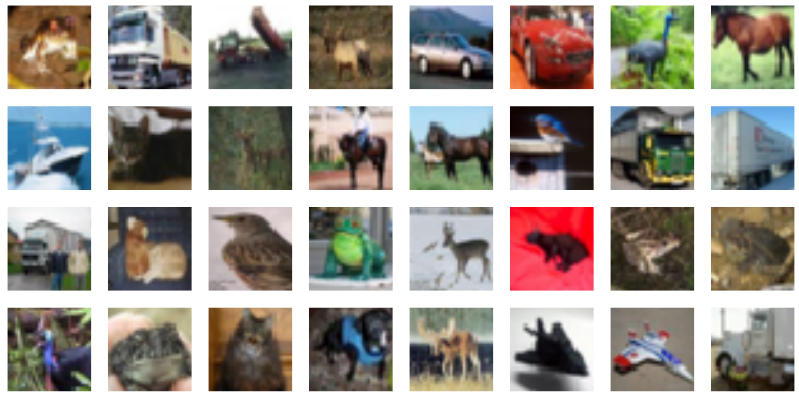
\includegraphics[width=0.75\textwidth]{./pic/cifar10_thermo_original.png}
    \end{figure}
  \end{minipage}\hfill%
  \begin{minipage}[h!]{0.5\textwidth}
    \begin{center}
      \bf CIFAR10 (generated)
    \end{center}
    \begin{figure}[h!]
      \centering
      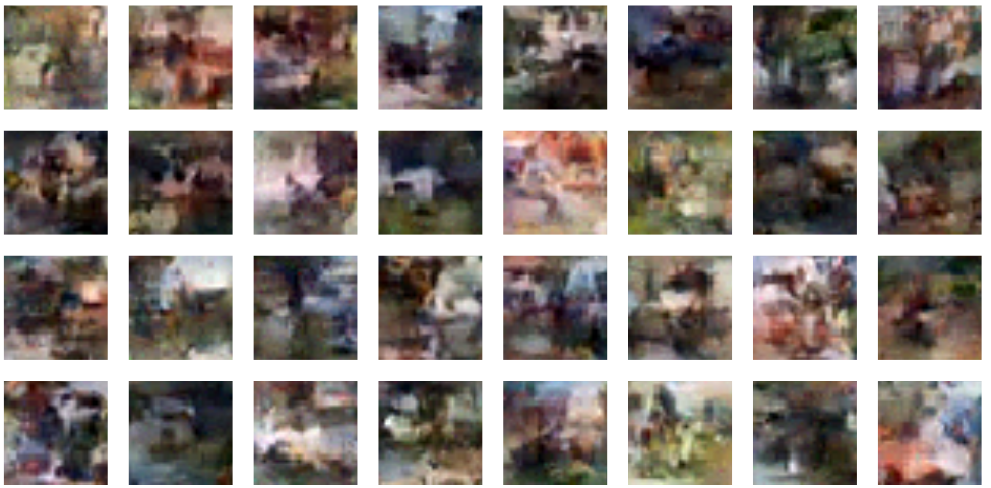
\includegraphics[width=0.75\textwidth]{./pic/cifar10_thermo_generated.png}
    \end{figure}
  \end{minipage}
\end{frame}

\begin{frame}{Timeline}
\begin{enumerate}
  \item[\bf 2015)] \textit{\ldots Non-equilibrium
  Thermodynamics}. Sohl-Dickstein et al. ICML. {\color{ggreen} \checkmark}\vfill
  \item[\bf 2020)] \textit{Denoising Diffusion Probabilistic Models}.
  Ho et al. NeurIPS.\vfill
  \item[\bf 2021)] \textit{Score-Based Generative Modeling Through SDE}. Song et
    al. ICLR.
\end{enumerate}
\end{frame}
\begin{frame}{Denoising Diffusion Probabilistic Model}
  \begin{center}
    \bf 
    Small technical improvements highly impact the
    performance\ldots\footcite{ho}
  \end{center}
  \begin{figure}[h]
    \centering
    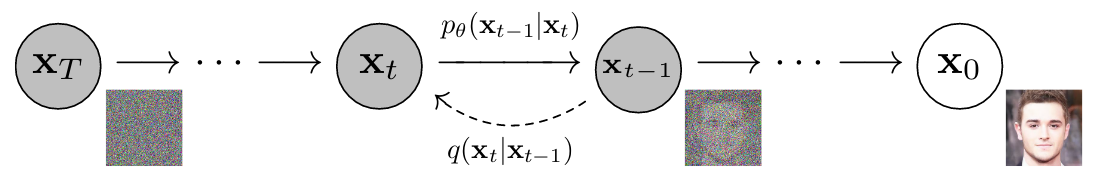
\includegraphics[width=0.75\textwidth]{./pic/ho_diffusion.png}
  \end{figure}
  \begin{block}{Simplification I: Diagonal Uniform Covariance
    Matrix}
    \[
      p_\theta(\xx^{(t-1)}\,\vert\,\xx^{(t)}) = \NN\left(\xx^{(t-1)};\, 
        \mub_\theta\left(
        \xx^{(t)},t \right),\, \Sigmab_\theta\left(\xx^{(t)},t \right)\right)
    \]
    where
    \[
      \Sigmab_\theta\left( \xx^{(t)},t  \right)= \sigma_t^2 I
    \]
  \end{block}
  \vfill
\end{frame}
\begin{frame}{Denoising Diffusion Probabilistic Model}
  \textbf{Previous work aims at estimating}
  \(
    \mub_\theta(\xx^{(t)},t)
  \) and
  \(
    \Sigmab_\theta(\xx^{(t)},t)
    \).
    \begin{block}{Simplification II: Estimating the commited error}
      \[
        \mub_\theta(\xx^{(t)})= \frac{1}{\sqrt{1-\beta_t}}\left( \xx^{(t)} -
          \frac{1-\beta_t}{\sqrt{\alpha_t}}\quad\onslide<2->{\tikzmarkin{a4}}\varepsilonb_\theta(\xx^{(t)},t)\onslide<2->{\tikzmarkend{a4}}
      \right)
      \]
    \onslide<2->{\tikzmarkin{a5} $\varepsilonb_\theta(\xx^{(t)},t)$ DNN
      (U-Net) with
      learnable parameters!!\tikzmarkend{a5}}
    \end{block}
      \vfill
    \onslide<3->{%
    \begin{block}{Simplification III: Training on random istants $t$}
      \[
        \LL_{simple} = \E_{t,\xx^{(0)},\varepsilonb}
        \left[ 
          \left\|\varepsilonb - \varepsilonb_\theta\left( \sqrt{1-\alpha_t}\xx^{(0)} + 
        \sqrt{\alpha_t}\varepsilonb,t \right)\right\| 
      \right]
      \]
      where
      \[
        t\sim \UU\left\{ 1,\ldots,T \right\},\quad \xx^{(0)}\sim q,\quad
        \varepsilon \sim \NN(0,I)
      \]
      \end{block}}
\end{frame}
\begin{frame}{Training and Sampling Procedure}
  \begin{figure}[h!]
    \centering
    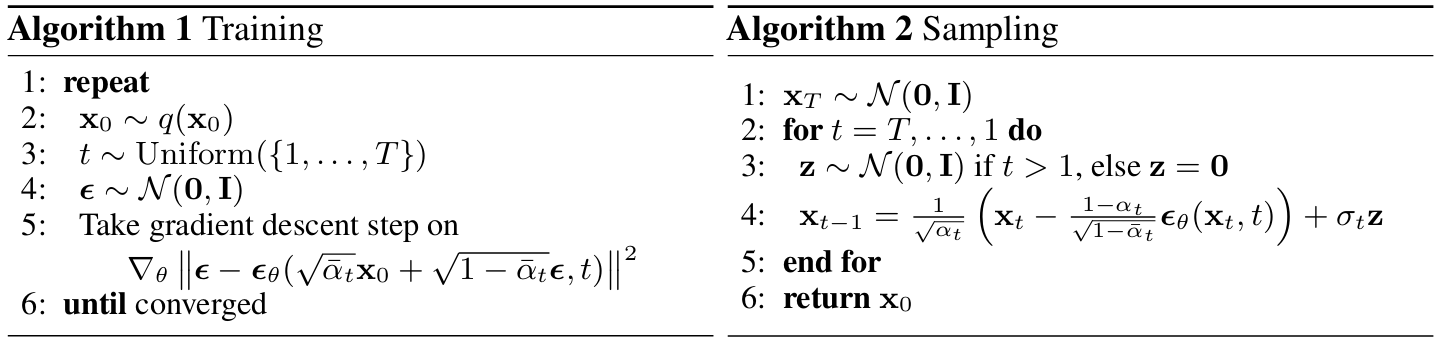
\includegraphics[width=0.6\textwidth]{./pic/ho_algo.png}
  \end{figure}
  \begin{figure}[h]
    \centering
    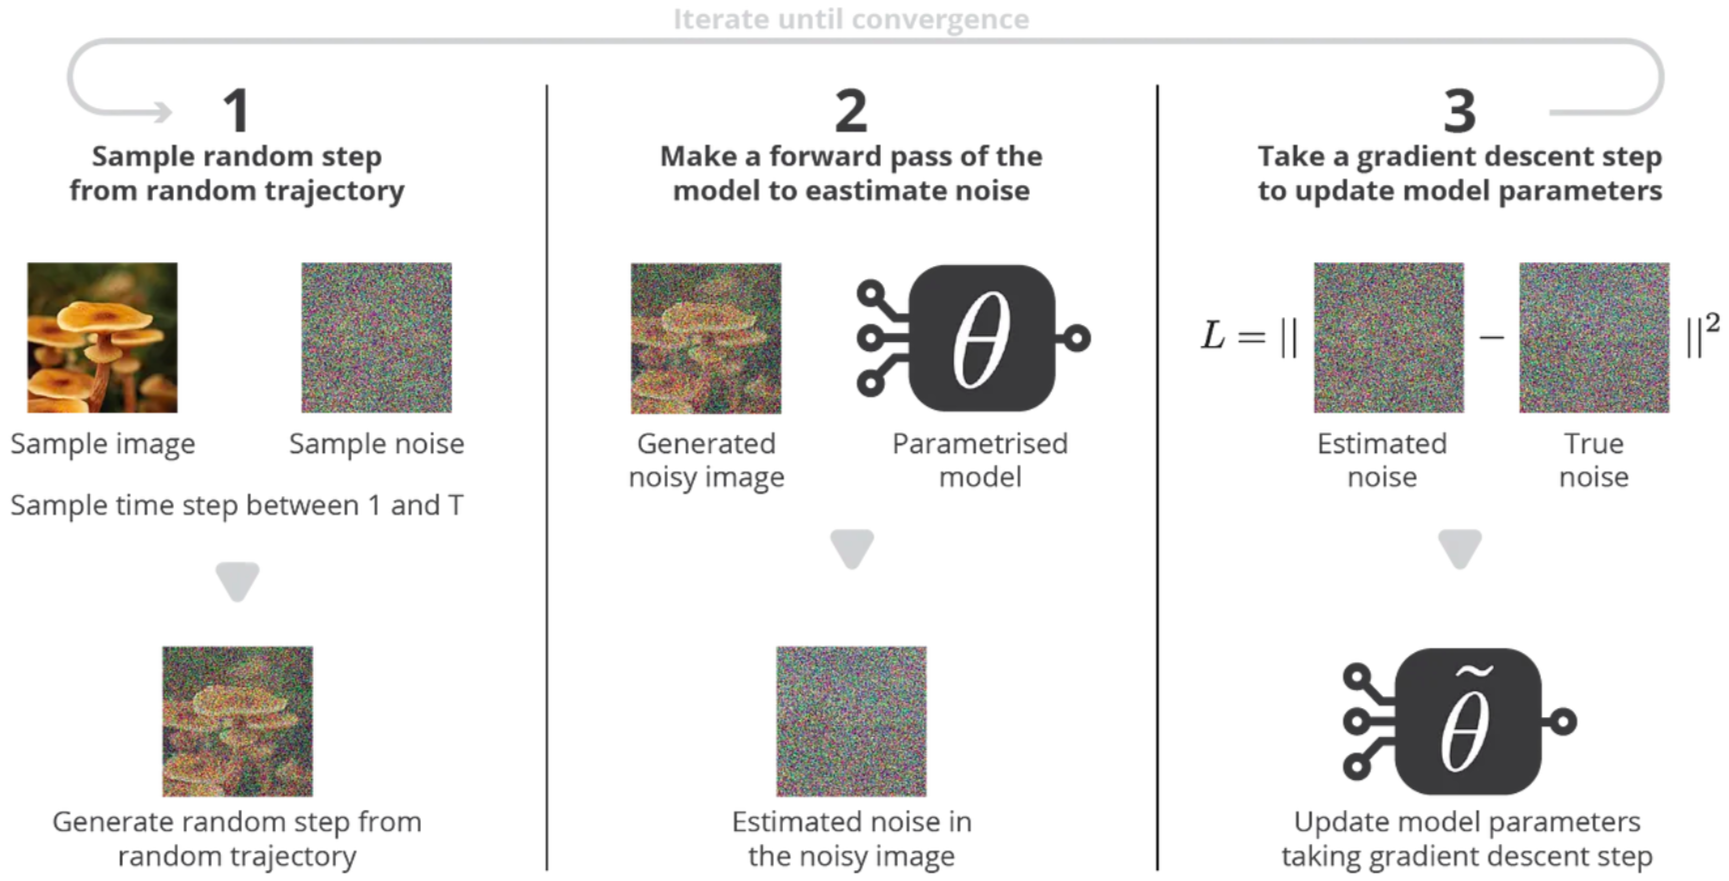
\includegraphics[width=0.60\textwidth]{./pic/ho_training.png}
    \caption{\footnote{\textbf{Credits}
    https://towardsdatascience.com/understanding-diffusion-probabilistic-models-dpms-1940329d6048}}
  \end{figure}
\end{frame}
\begin{frame}{Experiments: Sample Quality}
  \begin{minipage}[t]{0.6\textwidth}
    \begin{figure}[h!]
      \centering
      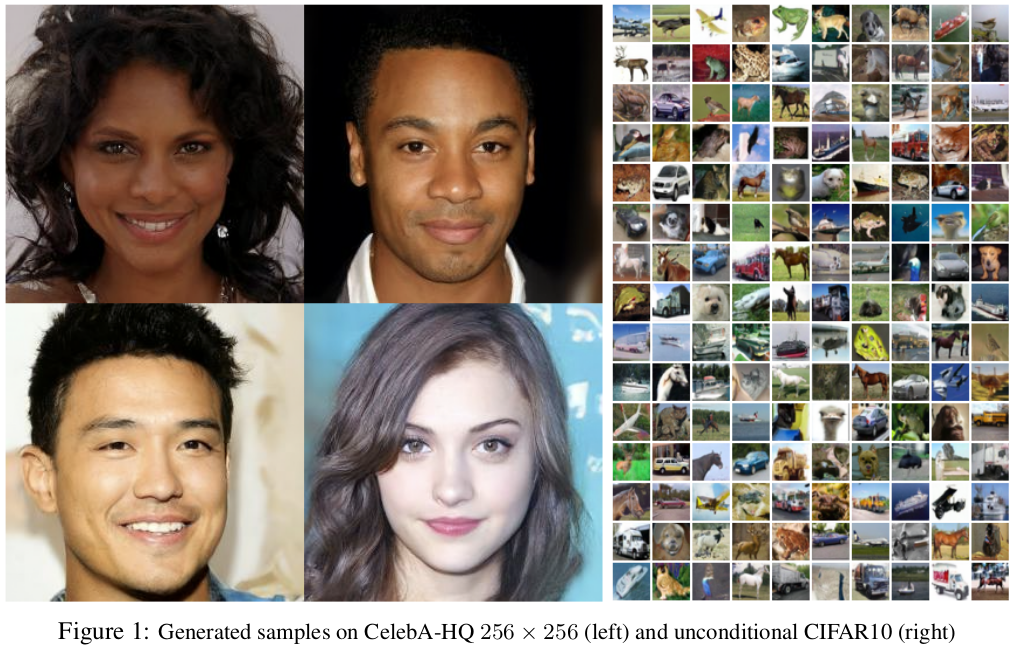
\includegraphics[width=\textwidth]{./pic/ho_celeb.png}
    \end{figure}
  \end{minipage}\hfill%
  \begin{minipage}[t]{0.35\textwidth}
    \begin{figure}[h]
      \centering
      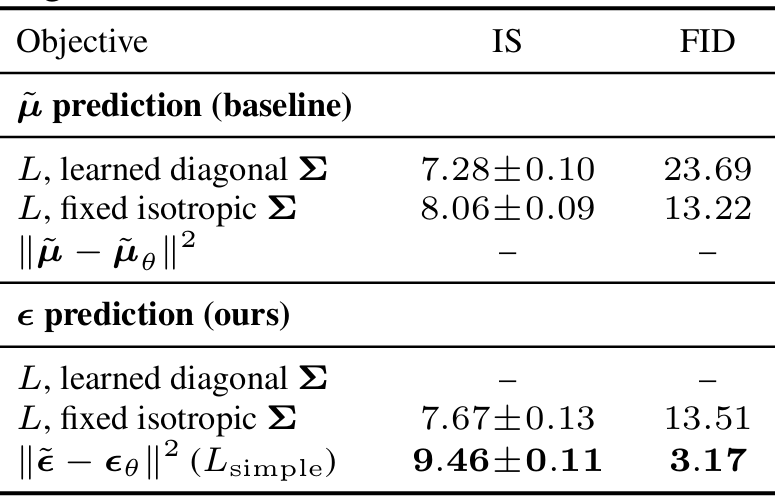
\includegraphics[width=\textwidth]{./pic/ho_result.png}
      \caption{Metrics for CIFAR10}
    \end{figure}
    \textbf{Note.}
    \begin{enumerate}
      \item Low FID (Frechet Implicit Distance) $\Rightarrow$ high quality 
      \item Training improved
    \end{enumerate}
  \end{minipage}

\end{frame}
\begin{frame}{Experiments: Diffusion vs GAN/VAE}
  \begin{center}
    \it ``Diffusion models get comparable result to Generative Adversarial
    Networks and Variational Autoencoders''
  \end{center}
  \begin{figure}[h]
    \centering
    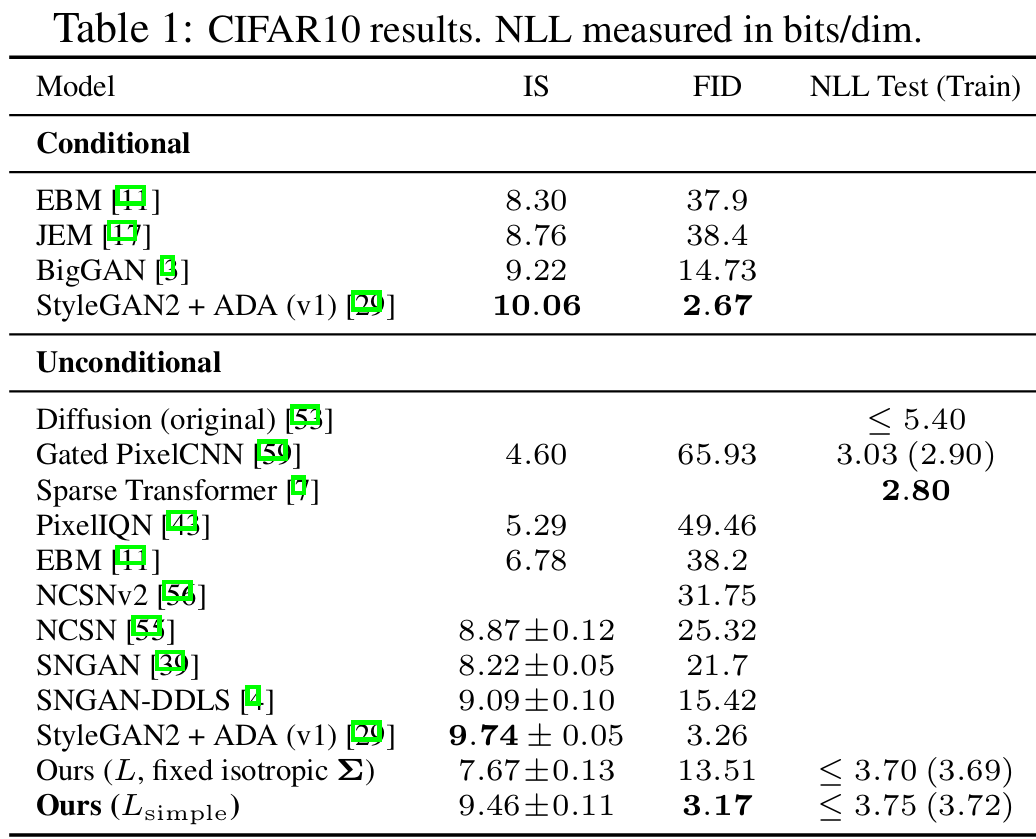
\includegraphics[width=0.4\textwidth]{{./pic/ho_table.png}}
    \caption{CIFAR10 results. NLL measured in bits/dim\footcite{ho}}
  \end{figure}%
\end{frame}

\begin{frame}{Experiments: Images Interpolation}
  \begin{figure}[h!]
    \centering
    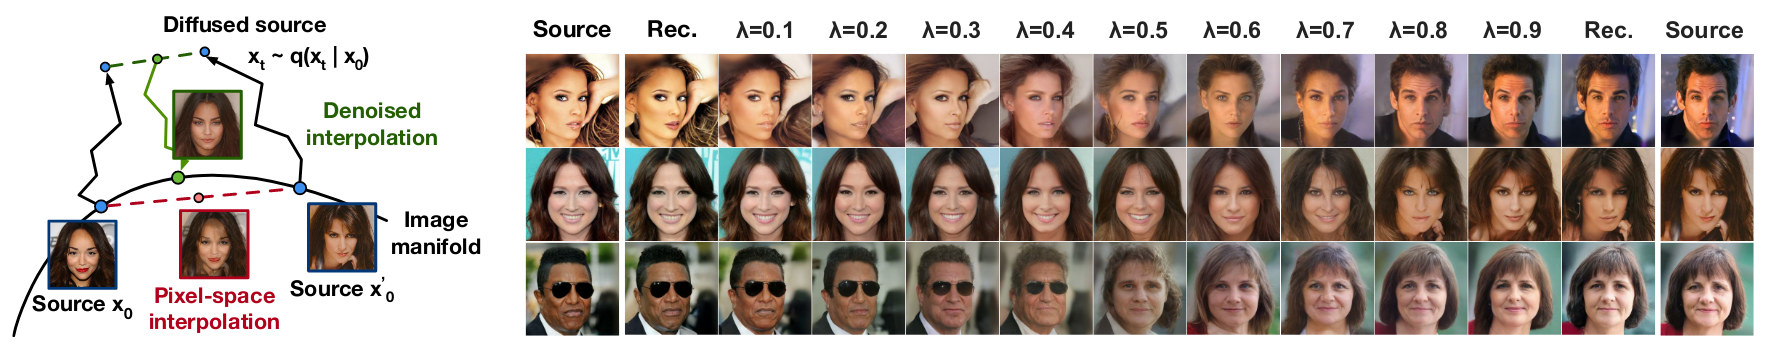
\includegraphics[width=\textwidth]{./pic/ho_interpolation.png}
  \end{figure}
  \[
    \xx^{(T)}_\lambda := \lambda\xx^{(T)}_{\tt source_r} +
    (1-\lambda)\xx^{(T)}_{\tt source_l},\quad \lambda\in\left[ 0,1
    \right]
  \]
  \pause
  \[
    \xx^{(0)}_\lambda \sim p_\theta(\xx^{(T)}),\quad \mbox{by diffusion}
  \]
\end{frame}
\begin{frame}{Timeline}
\begin{enumerate}
  \item[\bf 2015)] \textit{\ldots Non-equilibrium
  Thermodynamics}. Sohl-Dickstein et al. ICML. {\color{ggreen} \checkmark}\vfill
  \item[\bf 2020)] \textit{Denoising Diffusion Probabilistic Models}.
  Ho et al. NeurIPS.{\color{ggreen} \checkmark}\vfill
  \item[\bf 2021)] \textit{Score-Based Generative Modeling Through SDE}. Song et
    al. ICLR.
\end{enumerate}
\end{frame}
\begin{frame}{Score-Based Generative Modeling Through SDE (no details)}
  \begin{minipage}[h]{0.45\textwidth}
    \begin{center}
      \footnotesize 
      \textbf{Discrete Time}
    \end{center}
    \begin{figure}[h]
      \centering
      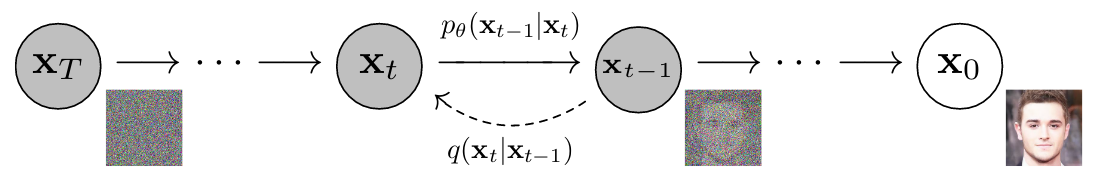
\includegraphics[width=\textwidth]{./pic/ho_diffusion.png}
    \end{figure}
  \end{minipage}\hfill%
  \begin{minipage}[h]{0.45\textwidth}
    \begin{center}
      \footnotesize 
      \textbf{\color{rred} Continuous Time}\\
    \end{center}
    \begin{figure}[h]
      \centering
      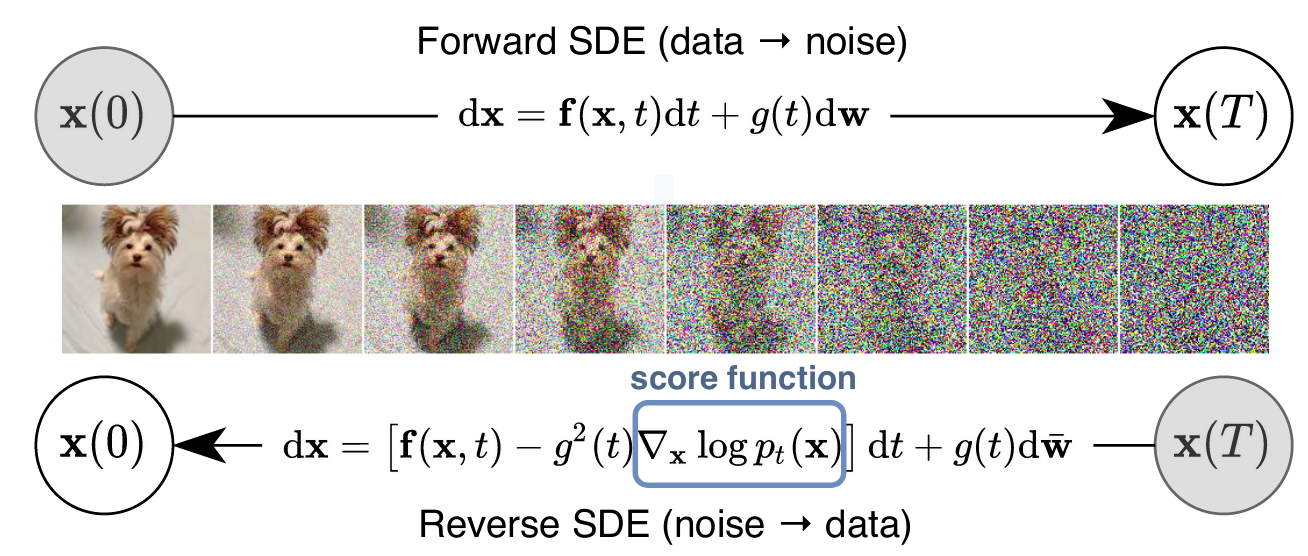
\includegraphics[width=\textwidth]{./pic/sda_intro.png}
    \end{figure}
  \end{minipage}\footcite{sde}
  \begin{block}{Stochastic Process}
    Continous sequence of $\xx$ indexed by $t\in\left[ 0,T \right]$, where $\xx(t)$ has distribution $p_t(\xx)$;
  \end{block}
\end{frame}
\begin{frame}{Continuous Diffusion Process described by SDE}
  %\begin{minipage}[t]{0.5\textwidth}
  %  \footnotesize
  %  \begin{center}
  %    \bf
  %    Discrete time Diffusion Process
  %  \end{center}
  %  \[
  %    \xx^{(t)}=\sqrt{1-\beta_t}\xx^{(t-1)} + \sqrt{\beta_t}
  %    \varepsilonb^{(t)}
  %  \]
  %  where $\varepsilonb\sim\NN(0,I)$.
  %\end{minipage}\hfill%
  \begin{minipage}[t]{0.5\textwidth}
    \begin{center}
      \bf
      Continous Diffusion Process
    \end{center}
    \[
      d\xx(t) = f(\xx,t) dt + g(t)\,d\ww(t)
    \]
    \begin{enumerate}
      \item $f(\xx,t)$ drift coefficient.
      \item $g(t)$ diffusion coefficient.
      \item $\ww(t)$, Weiner Process
    \end{enumerate}

    \begin{center}
      \bf
      Weiner Process
    \end{center}
      \[
        \ww(t)-\ww(s) \sim \NN(0,(t-s)I)
      \]
  \end{minipage}\hfill
  \begin{minipage}[t]{0.5\textwidth}
  \begin{figure}[h!]
    \centering
    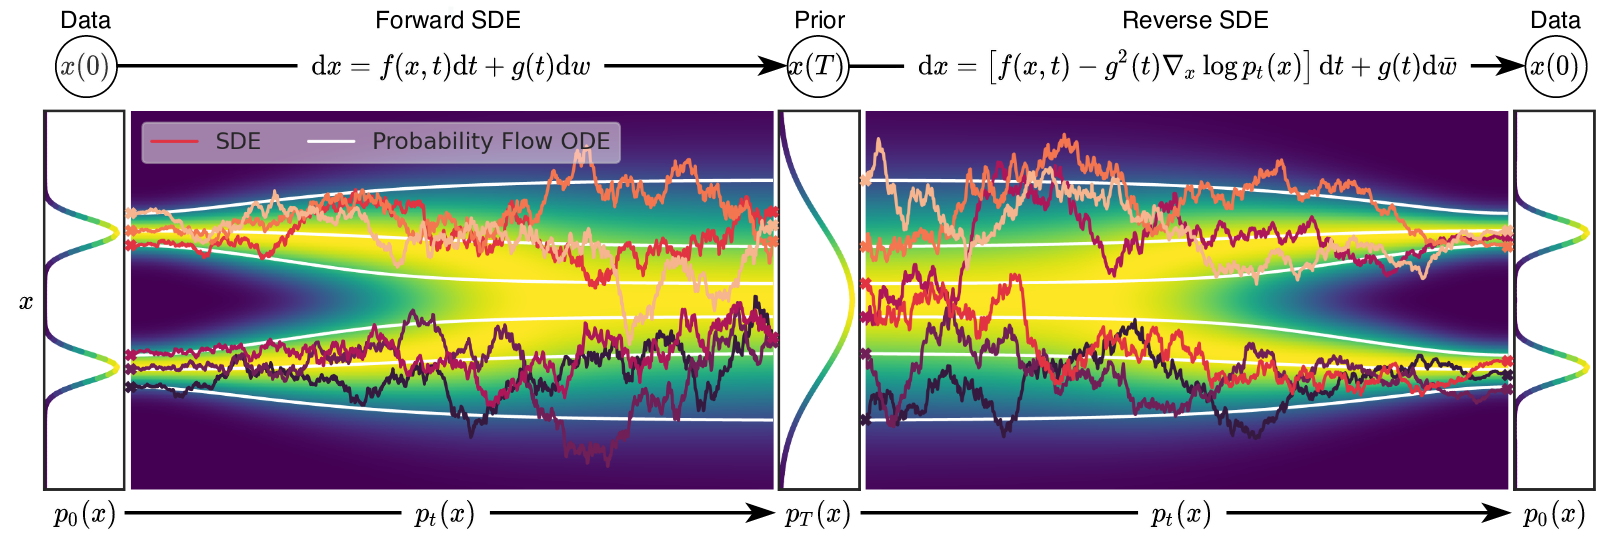
\includegraphics[clip, width=\textwidth,trim = 0 0 26.75cm 0]{./pic/sde_overview.png}
  \end{figure}
  \end{minipage}
\end{frame}
\begin{frame}{Reverse Process explicity given by $\nabla_{\xx} p_t(\xx)$}
  \begin{minipage}[t]{0.45\textwidth}
    \vspace{0.6cm}
    \begin{block}{Theorem}
      \footnotesize
      Reverse Process is still a diffusion process
      \[
        d\xx(t) = \bar f(\xx,t)\,dt + g(t)\,d\bar\ww(t)\\
      \]
      where
      \begin{itemize}
        \item $\bar f(\xx,t) = f(\xx,t) - g(t)^{2} \nabla_{\xx} log(p_t(\xx))$
          \item $\bar \ww(t)=\ww(T-t)$, reverse Weiner Process
      \end{itemize}
    \end{block}
  \end{minipage}\hfill
  \begin{minipage}[t]{0.5\textwidth}
  \begin{figure}[h!]
    \centering
    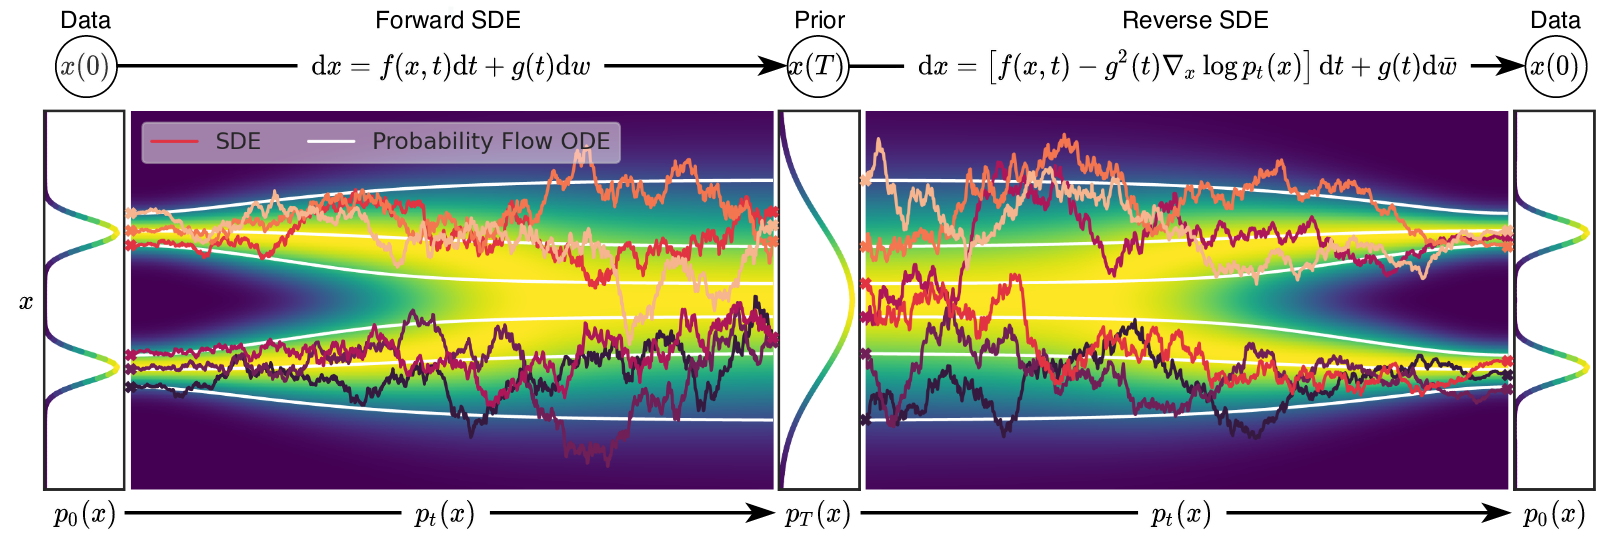
\includegraphics[clip, width=\textwidth,trim = 27.4cm 0 0 0]{./pic/sde_overview.png}
  \end{figure}
  \end{minipage}
\end{frame}
\section{DALL-E2}
\begin{frame}{Introduction}
  \begin{center}
    \bf
    A Ramesh et al. (Open AI). ``\textit{Hierarchical Text-Conditional Image 
    Generation with CLIP Latents.}''. February 2022.
  \end{center}
  \begin{minipage}[t]{0.5\textwidth}
  \begin{figure}[h!]
    \centering
    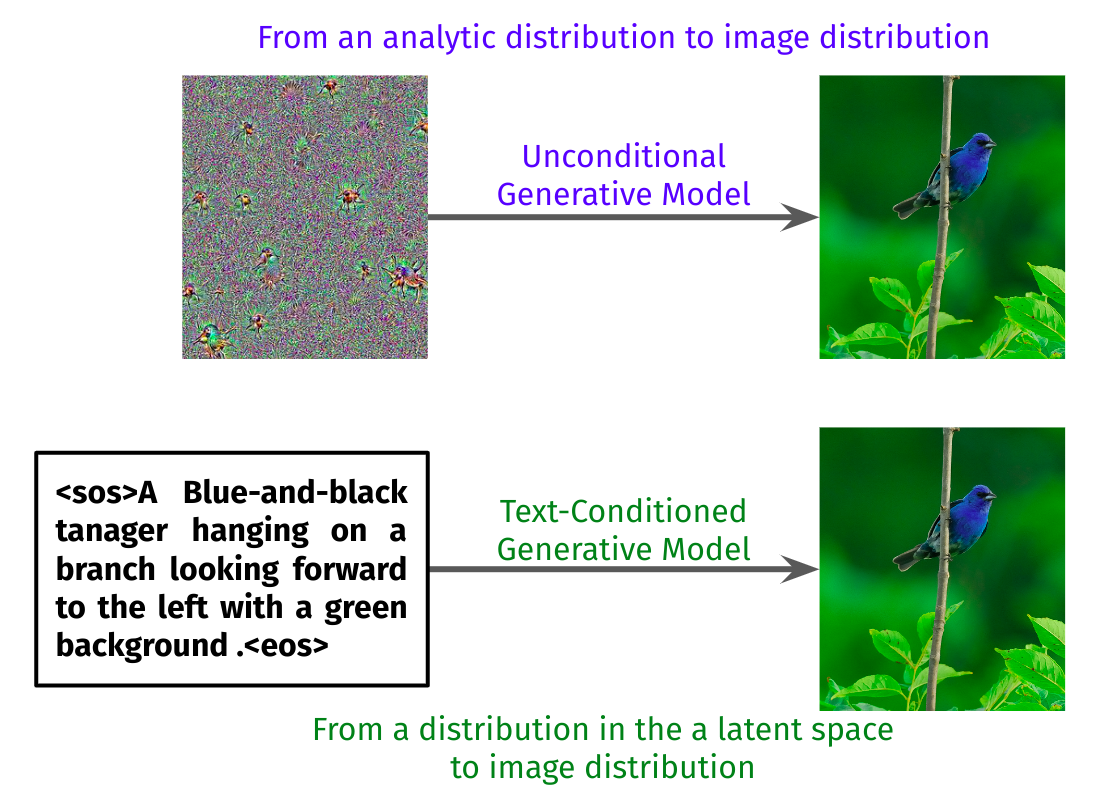
\includegraphics[width=\textwidth]{./pic/dalle-intro.png}
  \end{figure}
  \end{minipage}\hfill%
  \begin{minipage}[t]{0.5\textwidth}
    \begin{figure}[h]
      \centering
      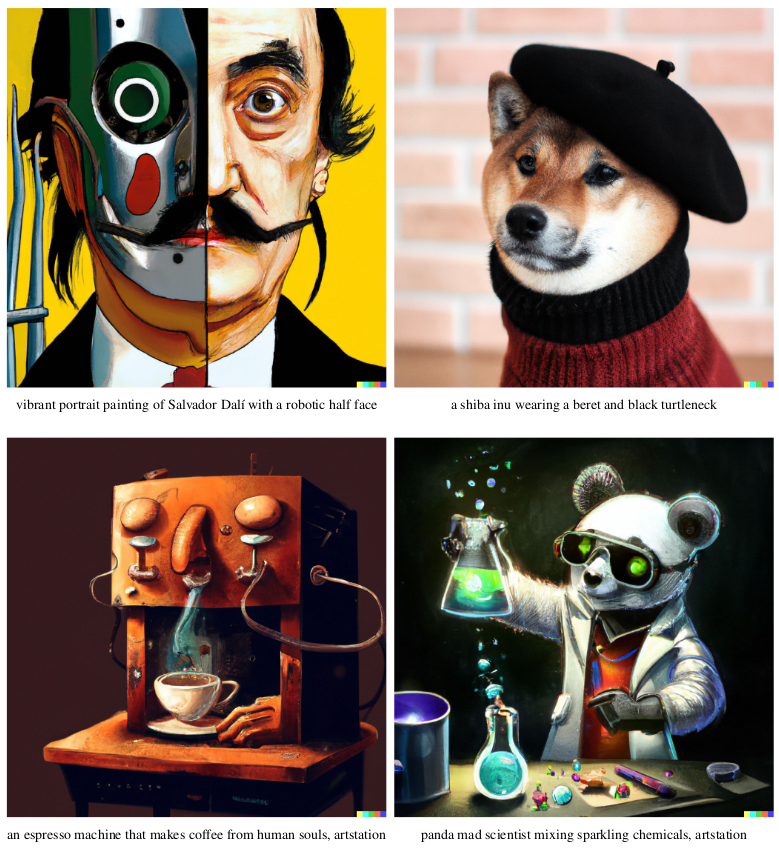
\includegraphics[width=0.75\textwidth]{./pic/dalle-samples.png}
    \end{figure}
  \end{minipage}
\end{frame}
\begin{frame}{Introduction}
  \begin{center}
    \bf\bf DALL-E2: a new AI system that can create realistic images and art from a 
    description in natural language
  \end{center}
  \begin{figure}[h]
    \centering
    \includegraphics<1>[clip, width=0.85\textwidth, trim=0 0 0 0]{./pic/dalle-samples2.png}%
    \includegraphics<2->[clip, width=0.85\textwidth, trim=0 0 0 1.25cm]{./pic/dalle-samples3.png}
    \caption{\footnote{\textbf{Credits:} DALL-E2 website}}
  \end{figure}
\end{frame}
\begin{frame}{Overview: CLIP + Diffusion}
  \begin{minipage}[t]{0.47\textwidth}
    \begin{center}
      \bf Text-to-Image Generation with CLIP
    \end{center}
    \begin{figure}[h]
      \centering
      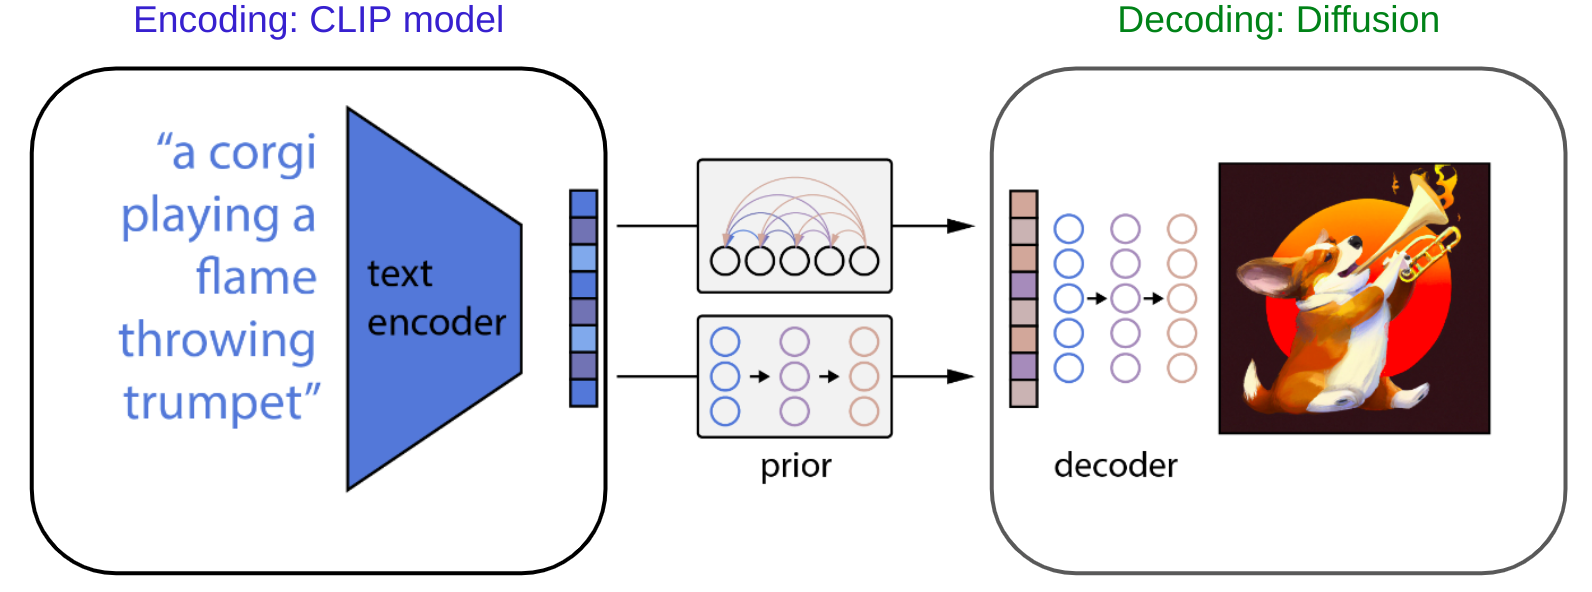
\includegraphics[width=1\textwidth]{./pic/dalle-encdec.png}
    \end{figure}
    \begin{center}
      Diffusion models allows generating images with  high sample fedelity
      and photorealism
    \end{center}
  \end{minipage}\hfill%
  \begin{minipage}[t]{0.47\textwidth}
    \begin{center}
      \bf CLIP model
    \end{center}
    \begin{figure}[h]
      \vspace{0.25cm}
      \centering
      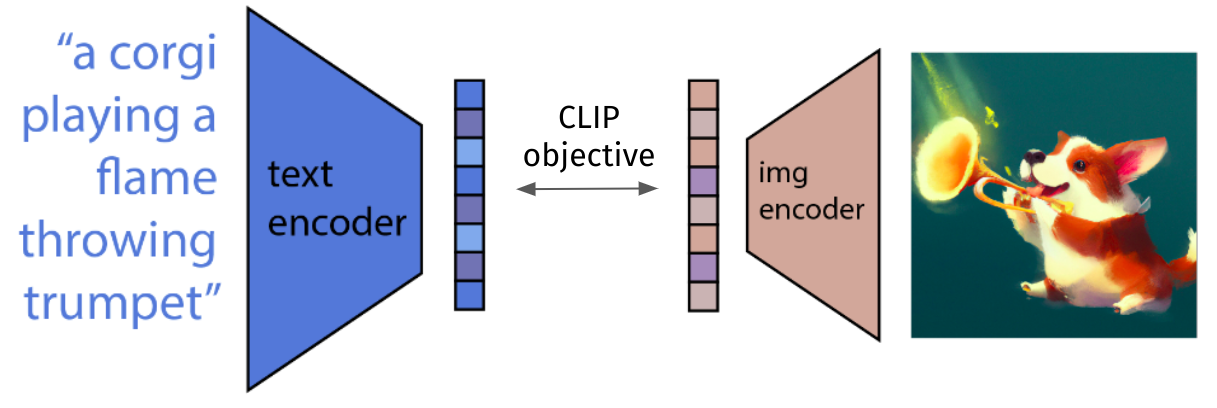
\includegraphics[width=\textwidth]{./pic/dalle-clip-intro.png}
    \end{figure}
  \begin{center}
    Embedding of images and text in the same latent space
  \end{center}
  \end{minipage}\hfill%
  \footcite{dalle2}
\end{frame}
\begin{frame}{CLIP: Latent Embedding model}
  \begin{columns}
  \begin{column}{0.5\textwidth}
    \only<1>{\begin{enumerate}
    \item  The \textbf{Text Encoder} takes as input a text $y$ in
      and embeds it in $z\in\R^n$.
      \vspace{0.5cm}
    \item The \textbf{Image Encoder} takes as input an image $x$ and embeds it in the
      latent space $\R^n$.
      \vspace{0.5cm}
    \item \textbf{Property}: The two embedded objects can be directly compared
      through cosine similarity.
    \end{enumerate}}
    \only<2->{\begin{enumerate}
        \item[4.] \textbf{Aim}: Zero-shot classification (of unseen
      datasets, see later.)
      \vspace{0.5cm}
        \item[5.]  The \textbf{Text Encoder} is a Transformer for NLP ($63M$ of
      parameters, next lectures).
      \vspace{0.5cm}
    \item[6.] The \textbf{Image Encoder} include ResNet-50 and Vision-Transformers
  \end{enumerate}}
  \end{column}
  \begin{column}{0.45\textwidth}
    \begin{figure}[t]
      \centering
      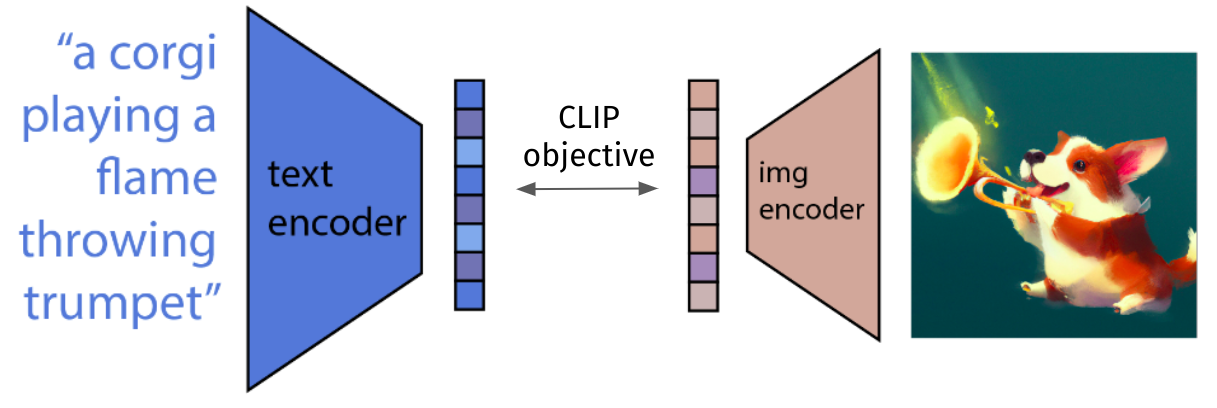
\includegraphics[width=\textwidth]{./pic/dalle-clip.png}
      \caption{CLIP allows embedding of images and text in the same latent
      space.}
    \end{figure}
  \end{column}
  \footcite{clip}
\end{columns}
\end{frame}
\begin{frame}{DALL-E2 with higher detail}
  \begin{figure}[h]
    \centering
    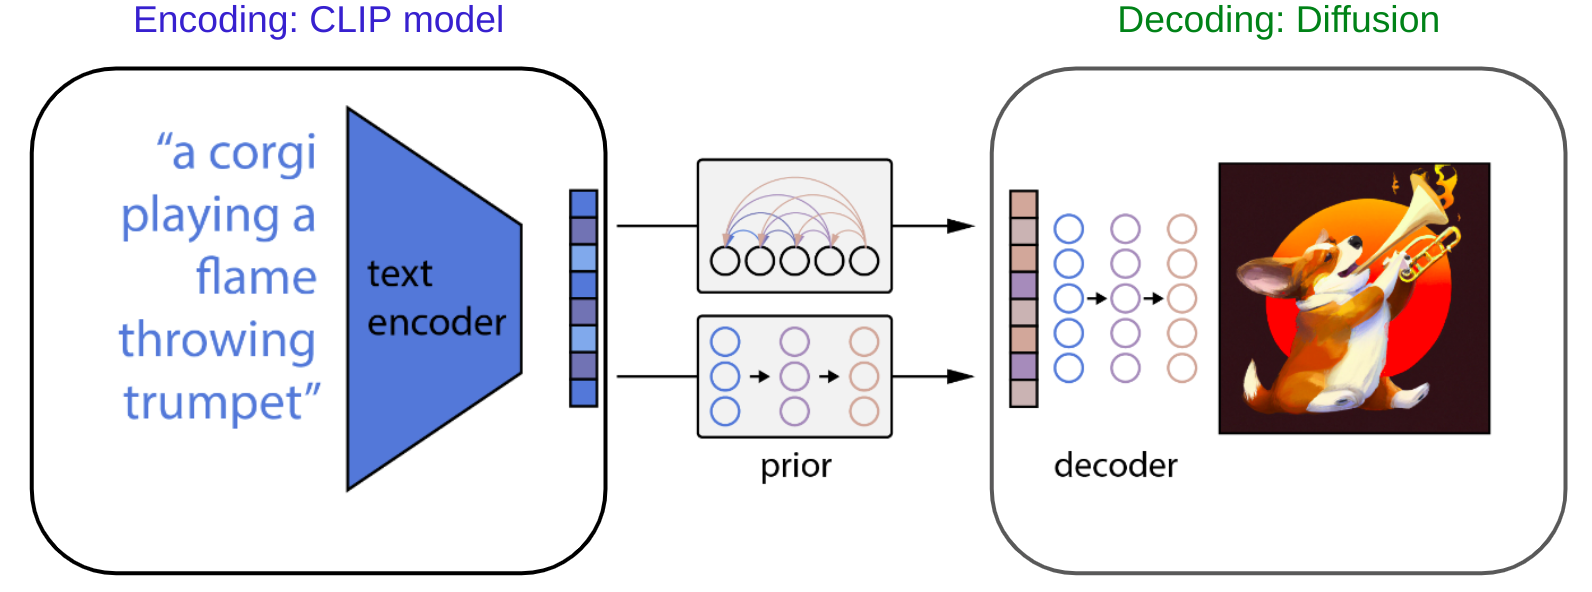
\includegraphics[width=0.5\textwidth]{./pic/dalle-encdec.png}
  \end{figure}
  Let $(x,y)$ be an (image, caption) pair.
  \begin{enumerate}
    \item \textbf{CLIP} such that $(x,y)\mapsto(z_i, z_t)$.
    \item \textbf{Prior} which estimates $q(\zz_i\,\vert\,\yy)$ \hfill
      \onslide<2->{\textit{\color{blue}Provide an image embedding conditioned
          to a text.}}
    \item \textbf{Decoder} which estimate $q(\xx\,\vert\, \zz_i,
      \yy)$\hfill
      \onslide<2->{\textit{\color{blue}Provide an Image conditioned to a
      text and Image Emb.}}
  \end{enumerate}
  \onslide<3->{
  \begin{block}{Observation}
    \[
      p(\xx\,\vert\, \yy) \underbrace{=}_{\mbox{\color{rred} Deterministic}}
      p(\xx,\zz_i\,\vert\,\yy) \underbrace{=}_{\mbox{\color{rred} Bayes Rule}} p(\xx\,\vert\,
      \zz_i,\yy)p(\zz_i\,\vert\,\yy)
    \]
\end{block}}
\end{frame}
\begin{frame}{Decoding through Diffusion models}
  \begin{columns}
    \begin{column}{0.5\textwidth}
      \begin{center}
        \textbf{Step 1: Generate a low-resolution image from $z_i$}\\
      A guided diffusion model is used to get a low resolution image from
      the image embedding.
      \end{center}
    \end{column}
    \begin{column}{0.5\textwidth}
      \onslide<2->{%
      \begin{center}
        \textbf{Step 2. Upsampling Procedure} \\
        Two diffusion models are used to increase the resolution of the image
        from low to super-high
      \end{center}}
    \end{column}
  \end{columns}
  \begin{figure}[h]
    \centering
    \includegraphics<1>[clip, width=\textwidth, trim = 0 8cm 0 10cm]{./pic/dalle-decoder_1.png}%
    \includegraphics<2->[clip, width=\textwidth, trim= 0 8cm 0 10cm]{./pic/dalle-decoder_2.png}
  \end{figure}
\end{frame}
\begin{frame}{Prior}
  \begin{center}
    \textbf{Diffusion Prior}: ``The image embedding $\zz_i$ is directly modelled 
    using a Gaussian diffusion model conditioned on the caption $\yy$''.
  \end{center}
  \begin{figure}[h!]
    \centering
    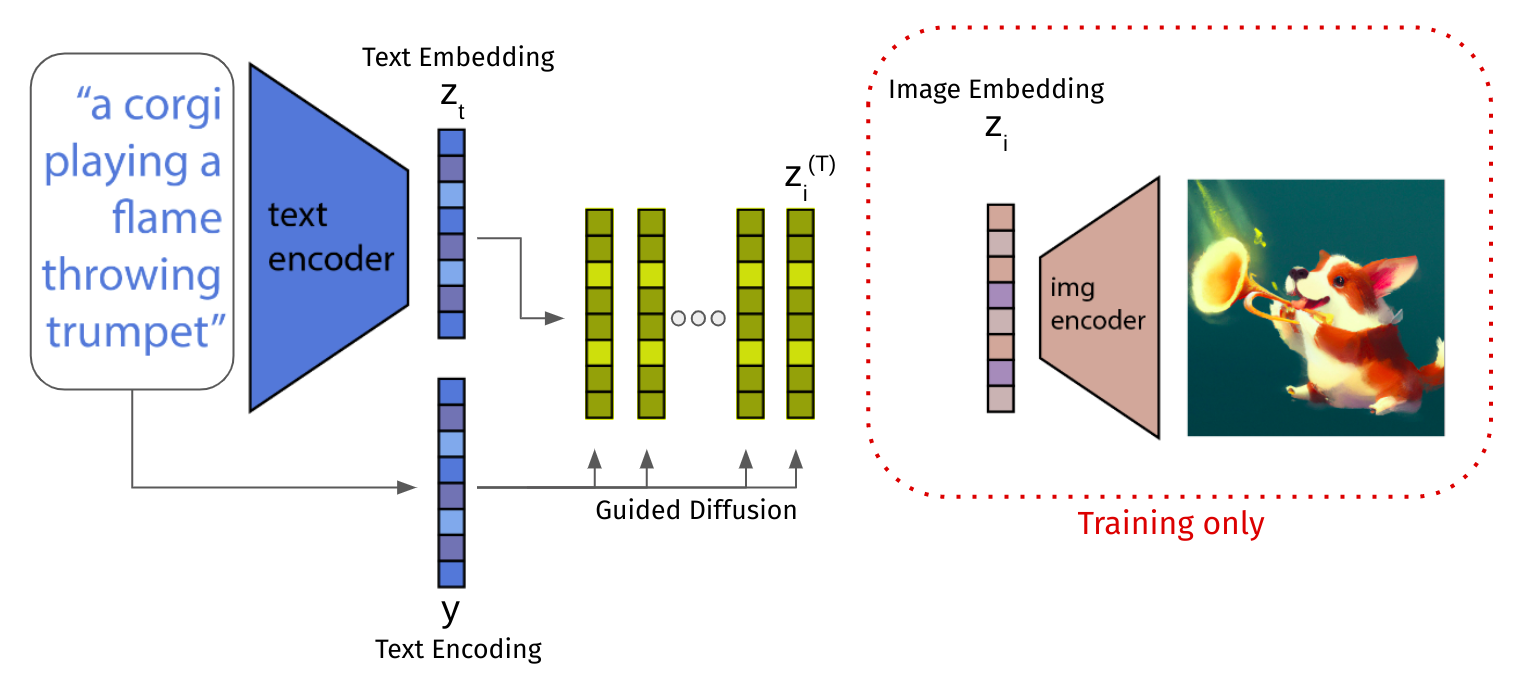
\includegraphics[width=0.75\textwidth]{./pic/dalle-prior.png}
  \end{figure}
  \textbf{Training Loss Function}
  \(
    L_{prior} = \E_{t\sim \left[ 1,T \right],\, \zz_i^{(t)} \sim q_t}
    \left[\|f_\theta(\zz_i^{(t)},\yy,t) - \zz_i\|^2  \right]
    \quad\mbox{where}\quad \zz_i^{(0)} = \zz_t
  \)
\end{frame}

\begin{frame}{Experiments:Image Interpolation}
  \begin{figure}[h]
    \centering
    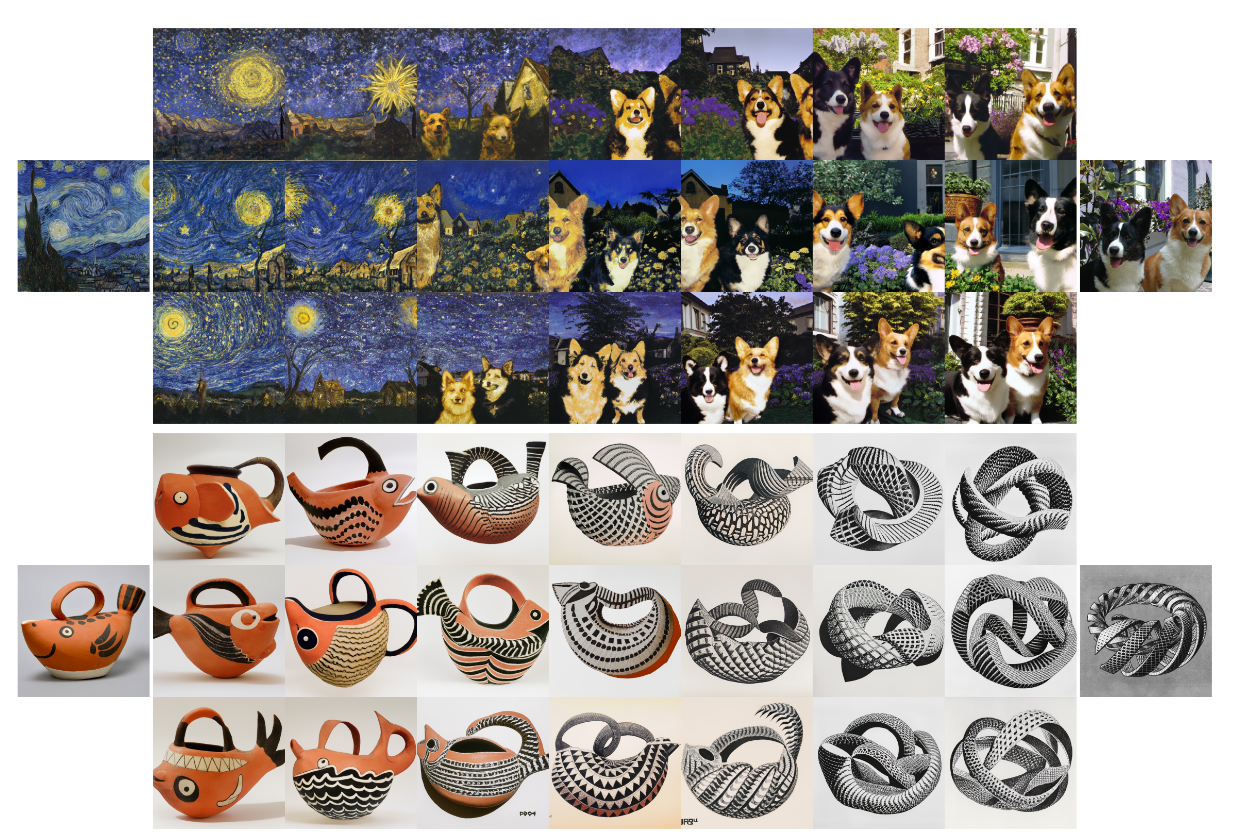
\includegraphics[width=0.75\textwidth]{./pic/dalle-image_interp.png}
    \caption{For each row, the decoder is applied to a combination of
    $\zz_i(left)$ and $\zz_i(right)$.}
  \end{figure}
\end{frame}
\begin{frame}{Experiments: Abstract Representation}
  \begin{center}
    \bf Representation of the Dignity
  \end{center}
  \begin{columns}
    \begin{column}{0.5\textwidth}
      \begin{figure}[h!]
        \centering
        \visible<2->{%
        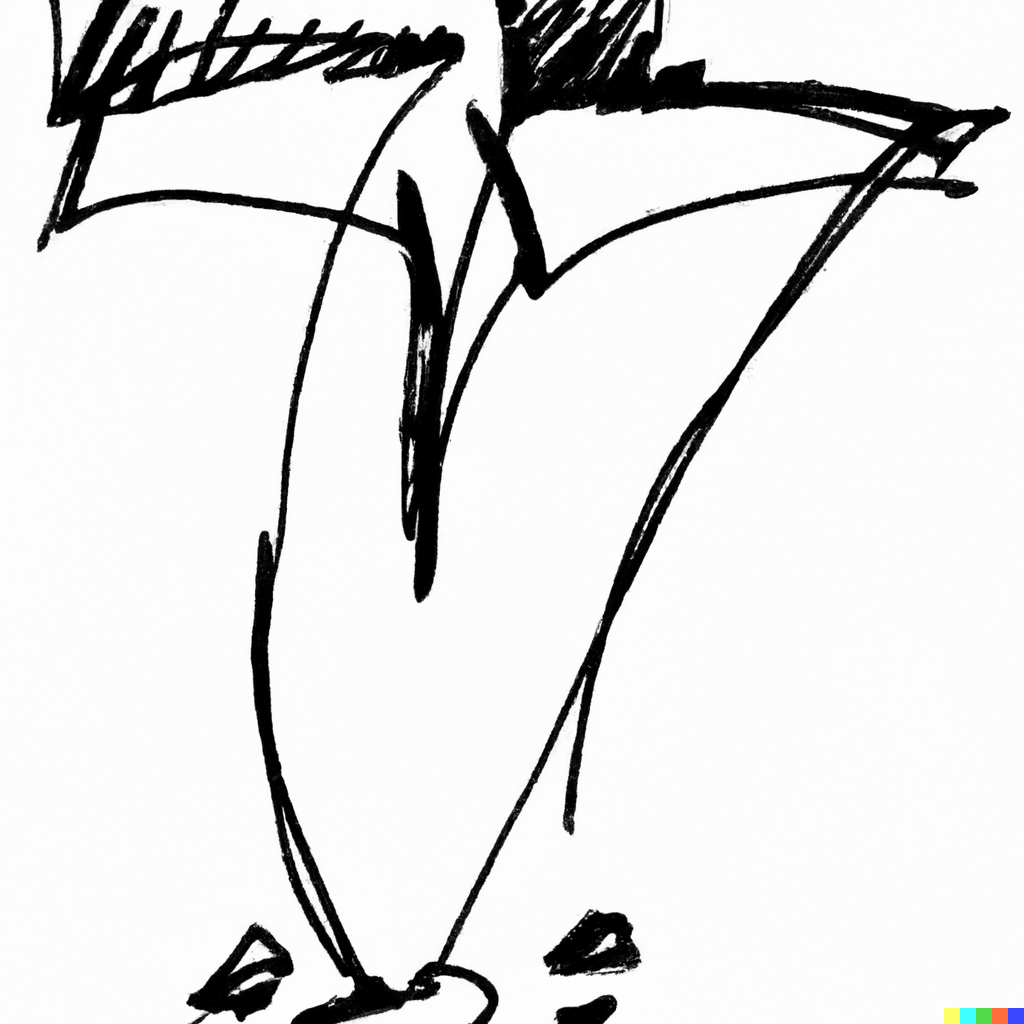
\includegraphics[width=0.75\textwidth]{./pic/dignity.png}
        \caption{\vspace{1pt}\bf DALL-E2}}
      \end{figure}
    \end{column}
    \begin{column}{0.5\textwidth}
      \begin{figure}[h!]
        \centering
        \visible<3->{%
        
\includegraphics[width=\textwidth]{./pic/Dignity-simposon.jpg}
      \caption{\vspace{1pt}\bf Matt Groening (S8 E6)}}
      \end{figure}
    \end{column}
  \end{columns}
\end{frame}
\begin{frame}{Experiments: Ricreate Anchient Works}
  \begin{columns}
    \begin{column}{0.5\textwidth}
      \begin{figure}[h]
        \centering
        
\includegraphics[width=0.9\textwidth]{./pic/anchient-work.png}
      \end{figure}
    \end{column}
    \begin{column}{0.5\textwidth}
      \begin{figure}[h]
        \centering
        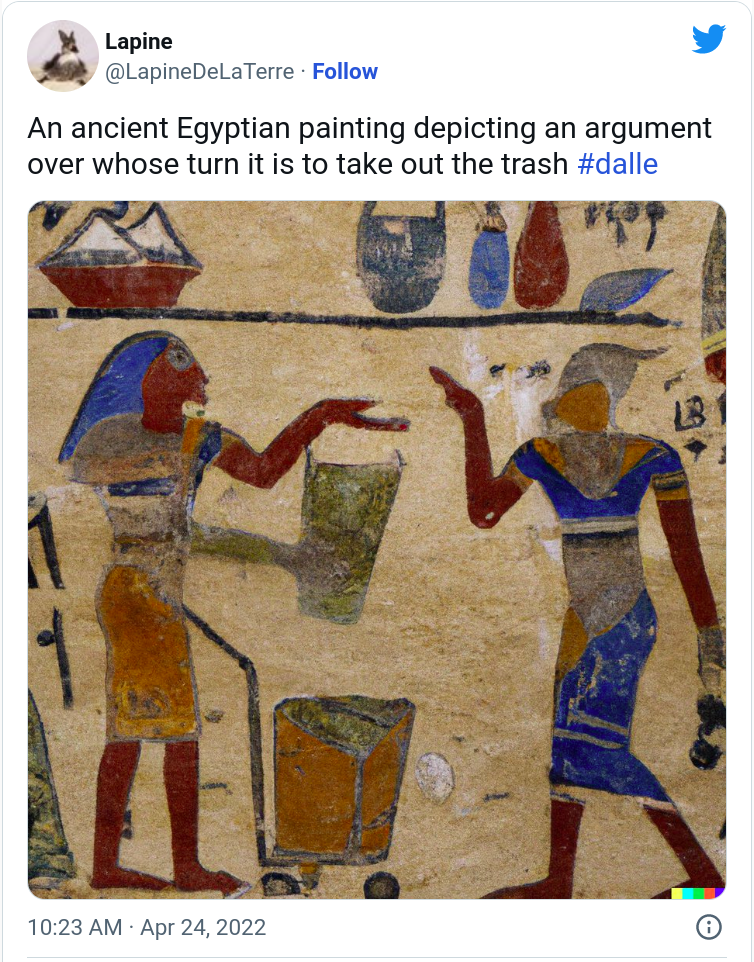
\includegraphics[width=0.8\textwidth]{./pic/trash-argue.png}
      \end{figure}
    \end{column}
  \end{columns}
\end{frame}
%\begin{frame}{Text Interpolation}
%  \begin{figure}[h]
%    \centering
%    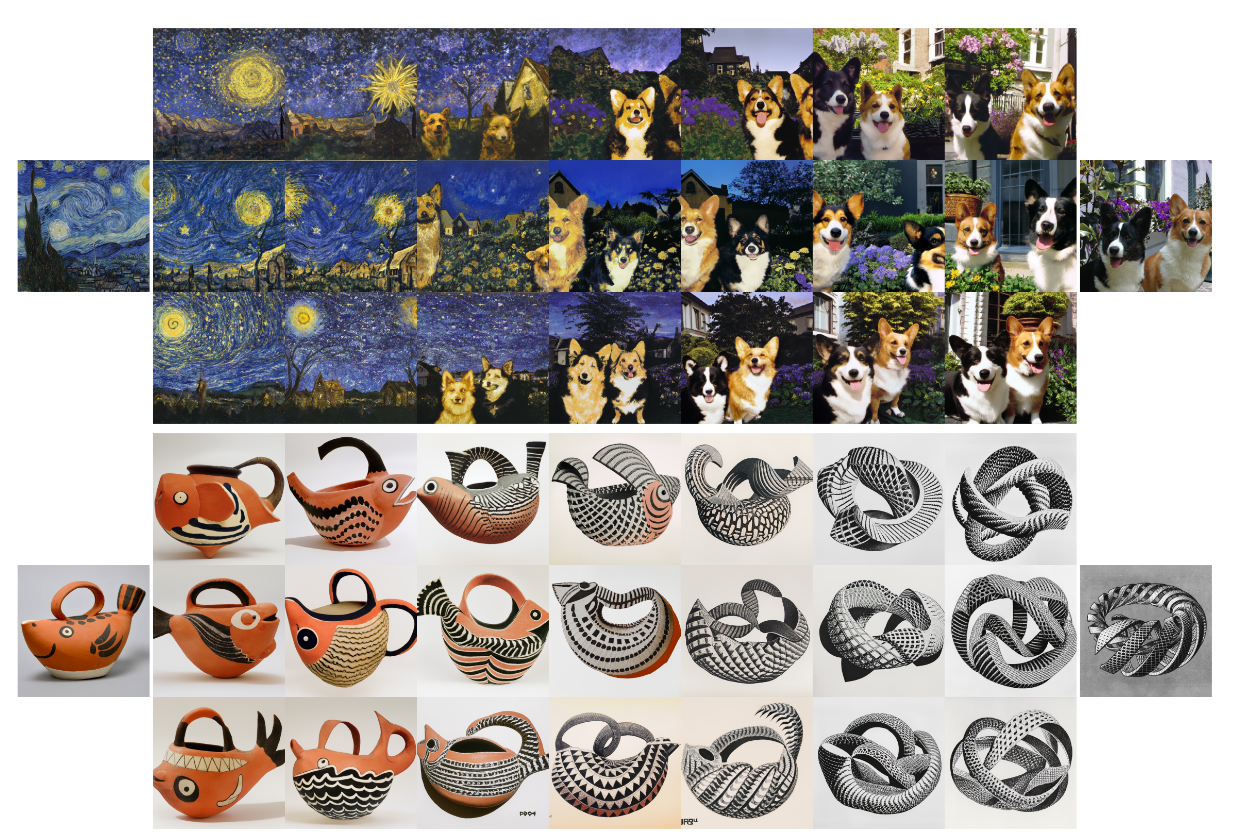
\includegraphics[width=0.75\textwidth]{./pic/dalle-image_interp.png}
%    \caption{For each row, the prior is applied to 
%    $\zz_i(left)$ and $\zz_i(right)$.}
%  \end{figure}
%
%\end{frame}
\section{Conclusion}
\begin{frame}{Broader Impacts}
  \begin{enumerate}
    \item Diffusion models, as generative models, can be used for malicious 
      porpouse. Fake images can become less detectable.
    \item Diffusion models reflects the biases in the dataset with which they
      are trained. Hence, using generated images for training other
      models can produce a \textbf{fade-in} effect.
  \end{enumerate}
  \pause
  \begin{center}
    \it``If samples from generative models trained on these datasets
    proliferate throughout the internet, then these biases will only be
    reinforced further.\footcite{ho}''
  \end{center}
\end{frame}
\begin{frame}{Summary}
  \begin{enumerate}
    \item Diffusion Generative Models (from 2015 to 2022)
      \vfill
    \item Overview on CLIP model for representation learning.
      \vfill
    \item The Diffusion models inside DALL-E2
  \end{enumerate}
\end{frame}
%\begin{frame}{CLIP Model}
%  \begin{center}
%    \it
%    ``We also found discrepancies across gender and race for people
%    categorized into the ‘crime’ and ‘non-human’
%    categories\ldots''\footcite{clip}
%  \end{center}
%\end{frame}
{%
  \setbeamercolor{background canvas}{bg=black!10!white}
  \setbeamertemplate{background}{%
  \begin{picture}(300,240)
    \hspace{0.9cm}
    
\includegraphics[scale=0.35]{pic/tecip_logo-ENG.png}
    \hspace{0.5cm}
    
\includegraphics[scale=0.17]{pic/dipe.png}
    \hspace{0.5cm}
    
\includegraphics[scale=0.085]{pic/logoretis.png}
  \end{picture}}
\begin{frame}{}
  \textbf{\Huge Thanks for the attention}\\
  \vspace{20pt}
  \begin{minipage}[h]{0.6\textwidth}
  {\large\bf Fabio Brau}
  \vspace{5pt}
  \begin{itemize}
    \item[\faUniversity] {\bf Scuola Superiore Sant'Anna, Pisa}
    \item[\Letter] \texttt{fabio.brau@santannapisa.it}
    \item[\faGlobe] \href{http://retis.santannapisa.it/~f.brau/}{\tt %
                    retis.santannapisa.it/\textasciitilde f.brau}
    \item[\faLinkedin]
      \href{https://www.linkedin.com/in/fabio-brau}{\tt%
        linkedin.com/in/fabio-brau}
  \end{itemize}
  \end{minipage}
\end{frame}
}

\appendix
\section{Proof Details}
\begin{frame}{Proof of Explicit Representation of Forward Diffusion Process}
  Let us proceeding by induction by assuming 
  $\xx^{(t)} = \sqrt{1-\alpha_t}\, \xx^{(0)} + \sqrt{\alpha_t}\,\varepsilonb$
  where $\varepsilonb\sim\NN(0,I)$ and where $\alpha_t =
  1-\prod_{i=0}^t(1-\beta_i)$. 
  \begin{equation}
    \begin{aligned}
      \xx^{(t+1)} &=  \sqrt{1-\beta_{t+1}}\, \xx^{(t)} +
      \sqrt{\beta_{t+1}}\,\varepsilonb_{t+1}\\
      &=\sqrt{1-\beta_{t+1}}\, \left(
      \sqrt{1-\alpha_t}\, \xx^{(0)} + \sqrt{\alpha_t}\,\varepsilonb\right) +
      \sqrt{\beta_{t+1}}\,\varepsilonb_{t+1}\\
      &= \sqrt{\left( \prod_{i=0}^{t+1}(1-\beta_i) \right)}\xx^{(0)} +
      \sqrt{(1-\beta_{t+1})\alpha_t+\beta_{t+1}}\,\tilde\varepsilonb
    \end{aligned}
  \end{equation}
    where the last term of the summation is obtained by observing that, since
    $\sqrt{(1-\beta_{t+1})\alpha_t}\,\varepsilonb$ and $\sqrt{\beta_{t+1}}\,\varepsilonb_{t+1}$ 
      are independent, then the variance of their sum (that still has a
      gaussian distribution) is given by
      $(1-\beta_{t+1})\alpha_t+ \beta_{t+1}$.
\end{frame}
\end{document}
\begin{frame}{Markov Chains with Discrete Time}
\textbf{Definition}\\ 
  A sequence of random variables $\left\{ \xx^{(t)}\right\}_{t\in\TT}
  \subseteq S$, such that the future $\xx^{(t+1)}$ depends on
  the present $\xx^{(t)}$ but not on the past $\xx^{(t-1)}$.\\
  \begin{itemize}
    \item \textbf{Discrete Time Property}\\
      \(
        \xx^{(0)},\,\xx^{(1)},\cdots,\xx^{(t)},\cdots 
      \)
    \item \textbf{Markov Property}\\
      \(
        \Ph\left( \xx^{(t+1)}\in A\,\vert\, \xx^{(0)},\ldots,\xx^{(t)}
        \right)=\Ph\left(\xx^{(t+1)}\in A\,\vert\,\xx^{(t)} \right)
      \)
  \end{itemize}
  \vfill
  \begin{minipage}[t]{0.4\textwidth}
    \begin{center}
      \textbf{Discrete State Space $S$}
    \end{center}
  \end{minipage}\hfill%
  \begin{minipage}[t]{0.4\textwidth}
    \begin{center}
      \textbf{Continuous State Space $S$}
    \end{center}
  \end{minipage}
\end{frame}
    \[
    D_{KL}\left( q(\xx^{(0)})||p_\theta(\xx^{)0)} \right) =
    \only<2>{\int q(\xx^{(0)})\log(q(\xx^{(0)})\,d\xx^{(0)}+
      \int-q(\xx^{(0)})\log(p_\theta(\xx^{(0)}))\,d\xx^{(0)}}
    \only<3->{\underbrace{\int q(\xx^{(0)})\log(q(\xx^{(0)})\,d\xx^{(0)}}_{-\Hh\left(
      q(\xx^{(0)}\right)} + 
    \underbrace{\int-q(\xx^{(0)})\log(p_\theta(\xx^{(0)}))\,d\xx^{(0)}}_{L_{CE}(p_\theta)}}
    \]
